% Options for packages loaded elsewhere
\PassOptionsToPackage{unicode}{hyperref}
\PassOptionsToPackage{hyphens}{url}
%
\documentclass[
]{article}
\usepackage{amsmath,amssymb}
\usepackage{lmodern}
\usepackage{iftex}
\ifPDFTeX
  \usepackage[T1]{fontenc}
  \usepackage[utf8]{inputenc}
  \usepackage{textcomp} % provide euro and other symbols
\else % if luatex or xetex
  \usepackage{unicode-math}
  \defaultfontfeatures{Scale=MatchLowercase}
  \defaultfontfeatures[\rmfamily]{Ligatures=TeX,Scale=1}
\fi
% Use upquote if available, for straight quotes in verbatim environments
\IfFileExists{upquote.sty}{\usepackage{upquote}}{}
\IfFileExists{microtype.sty}{% use microtype if available
  \usepackage[]{microtype}
  \UseMicrotypeSet[protrusion]{basicmath} % disable protrusion for tt fonts
}{}
\makeatletter
\@ifundefined{KOMAClassName}{% if non-KOMA class
  \IfFileExists{parskip.sty}{%
    \usepackage{parskip}
  }{% else
    \setlength{\parindent}{0pt}
    \setlength{\parskip}{6pt plus 2pt minus 1pt}}
}{% if KOMA class
  \KOMAoptions{parskip=half}}
\makeatother
\usepackage{xcolor}
\IfFileExists{xurl.sty}{\usepackage{xurl}}{} % add URL line breaks if available
\IfFileExists{bookmark.sty}{\usepackage{bookmark}}{\usepackage{hyperref}}
\hypersetup{
  pdftitle={STA Exam - MSBA Summer'22},
  pdfauthor={Prathmesh Savale, UTEID: ps33296},
  hidelinks,
  pdfcreator={LaTeX via pandoc}}
\urlstyle{same} % disable monospaced font for URLs
\usepackage[margin=1in]{geometry}
\usepackage{color}
\usepackage{fancyvrb}
\newcommand{\VerbBar}{|}
\newcommand{\VERB}{\Verb[commandchars=\\\{\}]}
\DefineVerbatimEnvironment{Highlighting}{Verbatim}{commandchars=\\\{\}}
% Add ',fontsize=\small' for more characters per line
\usepackage{framed}
\definecolor{shadecolor}{RGB}{248,248,248}
\newenvironment{Shaded}{\begin{snugshade}}{\end{snugshade}}
\newcommand{\AlertTok}[1]{\textcolor[rgb]{0.94,0.16,0.16}{#1}}
\newcommand{\AnnotationTok}[1]{\textcolor[rgb]{0.56,0.35,0.01}{\textbf{\textit{#1}}}}
\newcommand{\AttributeTok}[1]{\textcolor[rgb]{0.77,0.63,0.00}{#1}}
\newcommand{\BaseNTok}[1]{\textcolor[rgb]{0.00,0.00,0.81}{#1}}
\newcommand{\BuiltInTok}[1]{#1}
\newcommand{\CharTok}[1]{\textcolor[rgb]{0.31,0.60,0.02}{#1}}
\newcommand{\CommentTok}[1]{\textcolor[rgb]{0.56,0.35,0.01}{\textit{#1}}}
\newcommand{\CommentVarTok}[1]{\textcolor[rgb]{0.56,0.35,0.01}{\textbf{\textit{#1}}}}
\newcommand{\ConstantTok}[1]{\textcolor[rgb]{0.00,0.00,0.00}{#1}}
\newcommand{\ControlFlowTok}[1]{\textcolor[rgb]{0.13,0.29,0.53}{\textbf{#1}}}
\newcommand{\DataTypeTok}[1]{\textcolor[rgb]{0.13,0.29,0.53}{#1}}
\newcommand{\DecValTok}[1]{\textcolor[rgb]{0.00,0.00,0.81}{#1}}
\newcommand{\DocumentationTok}[1]{\textcolor[rgb]{0.56,0.35,0.01}{\textbf{\textit{#1}}}}
\newcommand{\ErrorTok}[1]{\textcolor[rgb]{0.64,0.00,0.00}{\textbf{#1}}}
\newcommand{\ExtensionTok}[1]{#1}
\newcommand{\FloatTok}[1]{\textcolor[rgb]{0.00,0.00,0.81}{#1}}
\newcommand{\FunctionTok}[1]{\textcolor[rgb]{0.00,0.00,0.00}{#1}}
\newcommand{\ImportTok}[1]{#1}
\newcommand{\InformationTok}[1]{\textcolor[rgb]{0.56,0.35,0.01}{\textbf{\textit{#1}}}}
\newcommand{\KeywordTok}[1]{\textcolor[rgb]{0.13,0.29,0.53}{\textbf{#1}}}
\newcommand{\NormalTok}[1]{#1}
\newcommand{\OperatorTok}[1]{\textcolor[rgb]{0.81,0.36,0.00}{\textbf{#1}}}
\newcommand{\OtherTok}[1]{\textcolor[rgb]{0.56,0.35,0.01}{#1}}
\newcommand{\PreprocessorTok}[1]{\textcolor[rgb]{0.56,0.35,0.01}{\textit{#1}}}
\newcommand{\RegionMarkerTok}[1]{#1}
\newcommand{\SpecialCharTok}[1]{\textcolor[rgb]{0.00,0.00,0.00}{#1}}
\newcommand{\SpecialStringTok}[1]{\textcolor[rgb]{0.31,0.60,0.02}{#1}}
\newcommand{\StringTok}[1]{\textcolor[rgb]{0.31,0.60,0.02}{#1}}
\newcommand{\VariableTok}[1]{\textcolor[rgb]{0.00,0.00,0.00}{#1}}
\newcommand{\VerbatimStringTok}[1]{\textcolor[rgb]{0.31,0.60,0.02}{#1}}
\newcommand{\WarningTok}[1]{\textcolor[rgb]{0.56,0.35,0.01}{\textbf{\textit{#1}}}}
\usepackage{graphicx}
\makeatletter
\def\maxwidth{\ifdim\Gin@nat@width>\linewidth\linewidth\else\Gin@nat@width\fi}
\def\maxheight{\ifdim\Gin@nat@height>\textheight\textheight\else\Gin@nat@height\fi}
\makeatother
% Scale images if necessary, so that they will not overflow the page
% margins by default, and it is still possible to overwrite the defaults
% using explicit options in \includegraphics[width, height, ...]{}
\setkeys{Gin}{width=\maxwidth,height=\maxheight,keepaspectratio}
% Set default figure placement to htbp
\makeatletter
\def\fps@figure{htbp}
\makeatother
\setlength{\emergencystretch}{3em} % prevent overfull lines
\providecommand{\tightlist}{%
  \setlength{\itemsep}{0pt}\setlength{\parskip}{0pt}}
\setcounter{secnumdepth}{-\maxdimen} % remove section numbering
\ifLuaTeX
  \usepackage{selnolig}  % disable illegal ligatures
\fi

\title{STA Exam - MSBA Summer'22}
\author{Prathmesh Savale, UTEID: ps33296}
\date{2022-07-24}

\begin{document}
\maketitle

These problems are done from the ISLR Edition 1 ebook.

\hypertarget{book-problems}{%
\section{Book Problems}\label{book-problems}}

\hypertarget{chapter-2}{%
\section{Chapter 2}\label{chapter-2}}

\hypertarget{question-10}{%
\subsubsection{Question 10}\label{question-10}}

\hypertarget{a-to-begin-load-in-the-boston-data-set.-the-boston-data-set-is}{%
\paragraph{(a) To begin, load in the Boston data set. The Boston data
set
is}\label{a-to-begin-load-in-the-boston-data-set.-the-boston-data-set-is}}

part of the MASS library in R. \textgreater{} library ( MASS) Now the
data set is contained in the object Boston. \textgreater{} Boston Read
about the data set: \textgreater{} ? Boston How many rows are in this
data set? How many columns? What do the rows and columns represent?

\begin{Shaded}
\begin{Highlighting}[]
\FunctionTok{rm}\NormalTok{(}\AttributeTok{list =} \FunctionTok{ls}\NormalTok{())}
\FunctionTok{library}\NormalTok{(tidyverse)}
\FunctionTok{library}\NormalTok{(ISLR)}
\FunctionTok{library}\NormalTok{(knitr)}
\FunctionTok{library}\NormalTok{(MASS)}
\FunctionTok{library}\NormalTok{(ggplot2)}
\FunctionTok{library}\NormalTok{(reshape2)}

\NormalTok{Boston }\SpecialCharTok{\%\textgreater{}\%}\NormalTok{ str}
\end{Highlighting}
\end{Shaded}

\begin{verbatim}
## 'data.frame':    506 obs. of  14 variables:
##  $ crim   : num  0.00632 0.02731 0.02729 0.03237 0.06905 ...
##  $ zn     : num  18 0 0 0 0 0 12.5 12.5 12.5 12.5 ...
##  $ indus  : num  2.31 7.07 7.07 2.18 2.18 2.18 7.87 7.87 7.87 7.87 ...
##  $ chas   : int  0 0 0 0 0 0 0 0 0 0 ...
##  $ nox    : num  0.538 0.469 0.469 0.458 0.458 0.458 0.524 0.524 0.524 0.524 ...
##  $ rm     : num  6.58 6.42 7.18 7 7.15 ...
##  $ age    : num  65.2 78.9 61.1 45.8 54.2 58.7 66.6 96.1 100 85.9 ...
##  $ dis    : num  4.09 4.97 4.97 6.06 6.06 ...
##  $ rad    : int  1 2 2 3 3 3 5 5 5 5 ...
##  $ tax    : num  296 242 242 222 222 222 311 311 311 311 ...
##  $ ptratio: num  15.3 17.8 17.8 18.7 18.7 18.7 15.2 15.2 15.2 15.2 ...
##  $ black  : num  397 397 393 395 397 ...
##  $ lstat  : num  4.98 9.14 4.03 2.94 5.33 ...
##  $ medv   : num  24 21.6 34.7 33.4 36.2 28.7 22.9 27.1 16.5 18.9 ...
\end{verbatim}

\begin{Shaded}
\begin{Highlighting}[]
\CommentTok{\# ?Boston}
\end{Highlighting}
\end{Shaded}

This data set has 506 rows and 14 columns. They represent the different
attributes associated with Boston housing data such as the crime rate by
town, average number of rooms per dwelling etc.

\hypertarget{b-make-some-pairwise-scatterplots-of-the-predictors-columns-in-this-data-set.-describe-your-findings.}{%
\paragraph{(b) Make some pairwise scatterplots of the predictors
(columns) in this data set. Describe your
findings.}\label{b-make-some-pairwise-scatterplots-of-the-predictors-columns-in-this-data-set.-describe-your-findings.}}

\begin{Shaded}
\begin{Highlighting}[]
\NormalTok{Boston }\SpecialCharTok{\%\textgreater{}\%} \FunctionTok{pairs}\NormalTok{()}
\end{Highlighting}
\end{Shaded}

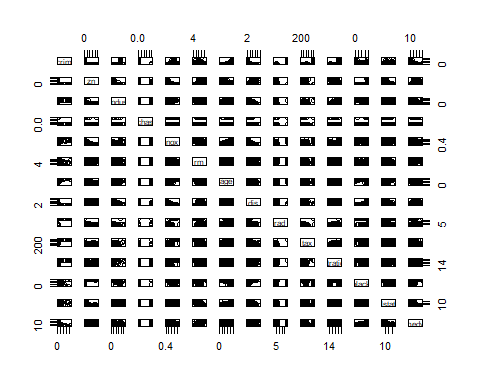
\includegraphics{STA_exam_ps33296_files/figure-latex/10.b-1.pdf}

\begin{itemize}
\tightlist
\item
  crime rate correlates with age, dis, rad, tax and ptratio
\item
  zn correlates with indus, nox, age, lstat and black
\item
  indus correlates with age and dis
\item
  lstat correlates with medv
\end{itemize}

\hypertarget{c-are-any-of-the-predictors-associated-with-per-capita-crime-rate-if-so-explain-the-relationship.}{%
\paragraph{(c) Are any of the predictors associated with per capita
crime rate? If so, explain the
relationship.}\label{c-are-any-of-the-predictors-associated-with-per-capita-crime-rate-if-so-explain-the-relationship.}}

\begin{Shaded}
\begin{Highlighting}[]
\NormalTok{df\_melt }\OtherTok{\textless{}{-}} \FunctionTok{melt}\NormalTok{(Boston,}\StringTok{"crim"}\NormalTok{)}
\CommentTok{\#scatterplot per group}
\FunctionTok{ggplot}\NormalTok{(df\_melt, }\FunctionTok{aes}\NormalTok{(crim,value)) }\SpecialCharTok{+}
  \FunctionTok{geom\_point}\NormalTok{() }\SpecialCharTok{+}
  \FunctionTok{facet\_grid}\NormalTok{(.}\SpecialCharTok{\textasciitilde{}}\NormalTok{variable)}
\end{Highlighting}
\end{Shaded}

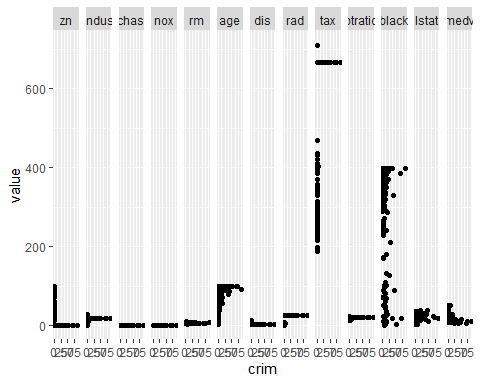
\includegraphics{STA_exam_ps33296_files/figure-latex/10.c-1.pdf}

\begin{itemize}
\tightlist
\item
  crime rate is higher in areas with higher property tax
\item
  crime rate is higher in areas where older people live
\item
  crime rate is higher where proportion of blacks is higher
\item
  crime rate is higher with higher pupil teacher ratio
\end{itemize}

\hypertarget{d-do-any-of-the-suburbs-of-boston-appear-to-have-particularly-high-crime-rates-tax-rates-pupil-teacher-ratios-comment-on-the-range-of-each-predictor.}{%
\paragraph{(d) Do any of the suburbs of Boston appear to have
particularly high crime rates? Tax rates? Pupil-teacher ratios? Comment
on the range of each
predictor.}\label{d-do-any-of-the-suburbs-of-boston-appear-to-have-particularly-high-crime-rates-tax-rates-pupil-teacher-ratios-comment-on-the-range-of-each-predictor.}}

\begin{Shaded}
\begin{Highlighting}[]
\NormalTok{Boston }\SpecialCharTok{\%\textgreater{}\%}\NormalTok{ summary}
\end{Highlighting}
\end{Shaded}

\begin{verbatim}
##       crim                zn             indus            chas        
##  Min.   : 0.00632   Min.   :  0.00   Min.   : 0.46   Min.   :0.00000  
##  1st Qu.: 0.08205   1st Qu.:  0.00   1st Qu.: 5.19   1st Qu.:0.00000  
##  Median : 0.25651   Median :  0.00   Median : 9.69   Median :0.00000  
##  Mean   : 3.61352   Mean   : 11.36   Mean   :11.14   Mean   :0.06917  
##  3rd Qu.: 3.67708   3rd Qu.: 12.50   3rd Qu.:18.10   3rd Qu.:0.00000  
##  Max.   :88.97620   Max.   :100.00   Max.   :27.74   Max.   :1.00000  
##       nox               rm             age              dis        
##  Min.   :0.3850   Min.   :3.561   Min.   :  2.90   Min.   : 1.130  
##  1st Qu.:0.4490   1st Qu.:5.886   1st Qu.: 45.02   1st Qu.: 2.100  
##  Median :0.5380   Median :6.208   Median : 77.50   Median : 3.207  
##  Mean   :0.5547   Mean   :6.285   Mean   : 68.57   Mean   : 3.795  
##  3rd Qu.:0.6240   3rd Qu.:6.623   3rd Qu.: 94.08   3rd Qu.: 5.188  
##  Max.   :0.8710   Max.   :8.780   Max.   :100.00   Max.   :12.127  
##       rad              tax           ptratio          black       
##  Min.   : 1.000   Min.   :187.0   Min.   :12.60   Min.   :  0.32  
##  1st Qu.: 4.000   1st Qu.:279.0   1st Qu.:17.40   1st Qu.:375.38  
##  Median : 5.000   Median :330.0   Median :19.05   Median :391.44  
##  Mean   : 9.549   Mean   :408.2   Mean   :18.46   Mean   :356.67  
##  3rd Qu.:24.000   3rd Qu.:666.0   3rd Qu.:20.20   3rd Qu.:396.23  
##  Max.   :24.000   Max.   :711.0   Max.   :22.00   Max.   :396.90  
##      lstat            medv      
##  Min.   : 1.73   Min.   : 5.00  
##  1st Qu.: 6.95   1st Qu.:17.02  
##  Median :11.36   Median :21.20  
##  Mean   :12.65   Mean   :22.53  
##  3rd Qu.:16.95   3rd Qu.:25.00  
##  Max.   :37.97   Max.   :50.00
\end{verbatim}

\begin{enumerate}
\def\labelenumi{\arabic{enumi}.}
\tightlist
\item
  areas with high black and high tax rate have higher crime rates
\item
  pt ratio doesnt affect the crime rate too much
\end{enumerate}

\begin{itemize}
\tightlist
\item
  range of crime rate - 88.87
\item
  range of tax rate - 524
\item
  range of ptratio - 9.4
\item
  range of black - 396.58
\item
  since the range of ptratio is less than crime rate, variation in it
  doesnt affect the crime rate much
\end{itemize}

\hypertarget{e-how-many-of-the-suburbs-in-this-data-set-bound-the-charles-river}{%
\paragraph{(e) How many of the suburbs in this data set bound the
Charles
river?}\label{e-how-many-of-the-suburbs-in-this-data-set-bound-the-charles-river}}

\begin{Shaded}
\begin{Highlighting}[]
\NormalTok{Boston }\SpecialCharTok{\%\textgreater{}\%} \FunctionTok{filter}\NormalTok{(chas }\SpecialCharTok{\textgreater{}} \DecValTok{0}\NormalTok{) }\SpecialCharTok{\%\textgreater{}\%} \FunctionTok{count}\NormalTok{()}
\end{Highlighting}
\end{Shaded}

\begin{verbatim}
##    n
## 1 35
\end{verbatim}

35 suburbs are bounded to river charles

\hypertarget{f-what-is-the-median-pupil-teacher-ratio-among-the-towns-in-this-data-set}{%
\paragraph{(f) What is the median pupil-teacher ratio among the towns in
this data
set?}\label{f-what-is-the-median-pupil-teacher-ratio-among-the-towns-in-this-data-set}}

\begin{Shaded}
\begin{Highlighting}[]
\NormalTok{Boston }\SpecialCharTok{\%\textgreater{}\%}\NormalTok{ str}
\end{Highlighting}
\end{Shaded}

\begin{verbatim}
## 'data.frame':    506 obs. of  14 variables:
##  $ crim   : num  0.00632 0.02731 0.02729 0.03237 0.06905 ...
##  $ zn     : num  18 0 0 0 0 0 12.5 12.5 12.5 12.5 ...
##  $ indus  : num  2.31 7.07 7.07 2.18 2.18 2.18 7.87 7.87 7.87 7.87 ...
##  $ chas   : int  0 0 0 0 0 0 0 0 0 0 ...
##  $ nox    : num  0.538 0.469 0.469 0.458 0.458 0.458 0.524 0.524 0.524 0.524 ...
##  $ rm     : num  6.58 6.42 7.18 7 7.15 ...
##  $ age    : num  65.2 78.9 61.1 45.8 54.2 58.7 66.6 96.1 100 85.9 ...
##  $ dis    : num  4.09 4.97 4.97 6.06 6.06 ...
##  $ rad    : int  1 2 2 3 3 3 5 5 5 5 ...
##  $ tax    : num  296 242 242 222 222 222 311 311 311 311 ...
##  $ ptratio: num  15.3 17.8 17.8 18.7 18.7 18.7 15.2 15.2 15.2 15.2 ...
##  $ black  : num  397 397 393 395 397 ...
##  $ lstat  : num  4.98 9.14 4.03 2.94 5.33 ...
##  $ medv   : num  24 21.6 34.7 33.4 36.2 28.7 22.9 27.1 16.5 18.9 ...
\end{verbatim}

\begin{Shaded}
\begin{Highlighting}[]
\NormalTok{median  }\OtherTok{=}\NormalTok{ Boston }\SpecialCharTok{\%\textgreater{}\%} 
\NormalTok{  dplyr}\SpecialCharTok{::}\FunctionTok{select}\NormalTok{(ptratio)  }\SpecialCharTok{\%\textgreater{}\%} 
  \FunctionTok{mutate}\NormalTok{(}\AttributeTok{Median =} \FunctionTok{median}\NormalTok{(ptratio))}

\NormalTok{median}\SpecialCharTok{$}\NormalTok{Median[}\DecValTok{1}\NormalTok{]}
\end{Highlighting}
\end{Shaded}

\begin{verbatim}
## [1] 19.05
\end{verbatim}

median is 19.05

\hypertarget{g-which-suburb-of-boston-has-lowest-median-value-of-owneroccupied-homes-what-are-the-values-of-the-other-predictors-for-that-suburb-and-how-do-those-values-compare-to-the-overall-ranges-for-those-predictors-comment-on-your-findings}{%
\paragraph{(g) Which suburb of Boston has lowest median value of
owneroccupied homes? What are the values of the other predictors for
that suburb, and how do those values compare to the overall ranges for
those predictors? Comment on your
findings}\label{g-which-suburb-of-boston-has-lowest-median-value-of-owneroccupied-homes-what-are-the-values-of-the-other-predictors-for-that-suburb-and-how-do-those-values-compare-to-the-overall-ranges-for-those-predictors-comment-on-your-findings}}

\begin{Shaded}
\begin{Highlighting}[]
\NormalTok{Boston }\SpecialCharTok{\%\textgreater{}\%} 
  \FunctionTok{filter}\NormalTok{(medv }\SpecialCharTok{==} \FunctionTok{min}\NormalTok{(medv))}
\end{Highlighting}
\end{Shaded}

\begin{verbatim}
##      crim zn indus chas   nox    rm age    dis rad tax ptratio  black lstat
## 1 38.3518  0  18.1    0 0.693 5.453 100 1.4896  24 666    20.2 396.90 30.59
## 2 67.9208  0  18.1    0 0.693 5.683 100 1.4254  24 666    20.2 384.97 22.98
##   medv
## 1    5
## 2    5
\end{verbatim}

\begin{Shaded}
\begin{Highlighting}[]
\CommentTok{\# there are 2 suburbs that have the least medv in the overall dataset.}
\NormalTok{Boston }\SpecialCharTok{\%\textgreater{}\%}\NormalTok{ summary}
\end{Highlighting}
\end{Shaded}

\begin{verbatim}
##       crim                zn             indus            chas        
##  Min.   : 0.00632   Min.   :  0.00   Min.   : 0.46   Min.   :0.00000  
##  1st Qu.: 0.08205   1st Qu.:  0.00   1st Qu.: 5.19   1st Qu.:0.00000  
##  Median : 0.25651   Median :  0.00   Median : 9.69   Median :0.00000  
##  Mean   : 3.61352   Mean   : 11.36   Mean   :11.14   Mean   :0.06917  
##  3rd Qu.: 3.67708   3rd Qu.: 12.50   3rd Qu.:18.10   3rd Qu.:0.00000  
##  Max.   :88.97620   Max.   :100.00   Max.   :27.74   Max.   :1.00000  
##       nox               rm             age              dis        
##  Min.   :0.3850   Min.   :3.561   Min.   :  2.90   Min.   : 1.130  
##  1st Qu.:0.4490   1st Qu.:5.886   1st Qu.: 45.02   1st Qu.: 2.100  
##  Median :0.5380   Median :6.208   Median : 77.50   Median : 3.207  
##  Mean   :0.5547   Mean   :6.285   Mean   : 68.57   Mean   : 3.795  
##  3rd Qu.:0.6240   3rd Qu.:6.623   3rd Qu.: 94.08   3rd Qu.: 5.188  
##  Max.   :0.8710   Max.   :8.780   Max.   :100.00   Max.   :12.127  
##       rad              tax           ptratio          black       
##  Min.   : 1.000   Min.   :187.0   Min.   :12.60   Min.   :  0.32  
##  1st Qu.: 4.000   1st Qu.:279.0   1st Qu.:17.40   1st Qu.:375.38  
##  Median : 5.000   Median :330.0   Median :19.05   Median :391.44  
##  Mean   : 9.549   Mean   :408.2   Mean   :18.46   Mean   :356.67  
##  3rd Qu.:24.000   3rd Qu.:666.0   3rd Qu.:20.20   3rd Qu.:396.23  
##  Max.   :24.000   Max.   :711.0   Max.   :22.00   Max.   :396.90  
##      lstat            medv      
##  Min.   : 1.73   Min.   : 5.00  
##  1st Qu.: 6.95   1st Qu.:17.02  
##  Median :11.36   Median :21.20  
##  Mean   :12.65   Mean   :22.53  
##  3rd Qu.:16.95   3rd Qu.:25.00  
##  Max.   :37.97   Max.   :50.00
\end{verbatim}

These have the highest number of elder population and high levels of
nox. And have higher levels of ptratio, black, and tax. These are not
the best places to live.

\hypertarget{h-in-this-data-set-how-many-of-the-suburbs-average-more-than-seven-rooms-per-dwelling-more-than-eight-rooms-per-dwelling-comment-on-the-suburbs-that-average-more-than-eight-rooms-per-dwelling.}{%
\paragraph{(h) In this data set, how many of the suburbs average more
than seven rooms per dwelling? More than eight rooms per dwelling?
Comment on the suburbs that average more than eight rooms per
dwelling.}\label{h-in-this-data-set-how-many-of-the-suburbs-average-more-than-seven-rooms-per-dwelling-more-than-eight-rooms-per-dwelling-comment-on-the-suburbs-that-average-more-than-eight-rooms-per-dwelling.}}

\begin{Shaded}
\begin{Highlighting}[]
\NormalTok{Boston }\SpecialCharTok{\%\textgreater{}\%} 
  \FunctionTok{filter}\NormalTok{(rm }\SpecialCharTok{\textgreater{}} \DecValTok{7}\NormalTok{) }\SpecialCharTok{\%\textgreater{}\%} \FunctionTok{count}\NormalTok{()}
\end{Highlighting}
\end{Shaded}

\begin{verbatim}
##    n
## 1 64
\end{verbatim}

\begin{Shaded}
\begin{Highlighting}[]
\CommentTok{\# 64 suburbs average more than 7 rooms per dwelling}

\NormalTok{Boston }\SpecialCharTok{\%\textgreater{}\%} 
  \FunctionTok{filter}\NormalTok{(rm }\SpecialCharTok{\textgreater{}} \DecValTok{7}\NormalTok{) }\SpecialCharTok{\%\textgreater{}\%} \FunctionTok{boxplot}\NormalTok{()}
\end{Highlighting}
\end{Shaded}

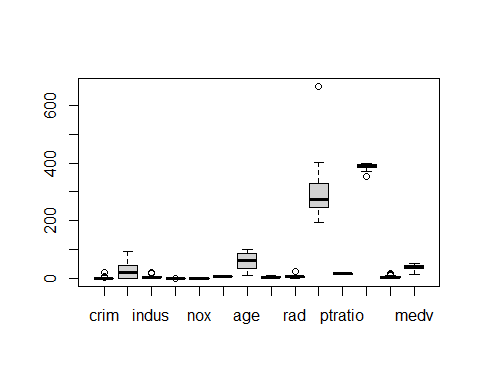
\includegraphics{STA_exam_ps33296_files/figure-latex/10.h-1.pdf}

\begin{Shaded}
\begin{Highlighting}[]
\NormalTok{Boston }\SpecialCharTok{\%\textgreater{}\%} 
  \FunctionTok{filter}\NormalTok{(rm }\SpecialCharTok{\textgreater{}} \DecValTok{8}\NormalTok{) }\SpecialCharTok{\%\textgreater{}\%} \FunctionTok{count}\NormalTok{()}
\end{Highlighting}
\end{Shaded}

\begin{verbatim}
##    n
## 1 13
\end{verbatim}

\begin{Shaded}
\begin{Highlighting}[]
\CommentTok{\# 13 suburbs average more than 8 rooms per dwelling}

\NormalTok{Boston }\SpecialCharTok{\%\textgreater{}\%} 
  \FunctionTok{filter}\NormalTok{(rm }\SpecialCharTok{\textgreater{}} \DecValTok{8}\NormalTok{) }\SpecialCharTok{\%\textgreater{}\%} \FunctionTok{boxplot}\NormalTok{()}
\end{Highlighting}
\end{Shaded}

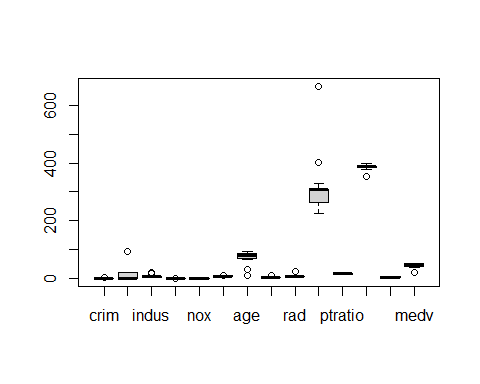
\includegraphics{STA_exam_ps33296_files/figure-latex/10.h-2.pdf}

\begin{Shaded}
\begin{Highlighting}[]
\CommentTok{\# the taxes and medv on these homes are on the higher side}
\CommentTok{\# compared to more than 7 rooms per dwelling}
\end{Highlighting}
\end{Shaded}

\begin{center}\rule{0.5\linewidth}{0.5pt}\end{center}

\hypertarget{chapter-3}{%
\section{Chapter 3}\label{chapter-3}}

\hypertarget{question-15}{%
\subsubsection{Question 15}\label{question-15}}

This problem involves the Boston data set, which we saw in the lab for
this chapter. We will now try to predict per capita crime rate using the
other variables in this data set. In other words, per capita crime rate
is the response, and the other variables are the predictors

\hypertarget{a-for-each-predictor-fit-a-simple-linear-regression-model-to-predict}{%
\paragraph{(a) For each predictor, fit a simple linear regression model
to
predict}\label{a-for-each-predictor-fit-a-simple-linear-regression-model-to-predict}}

the response. Describe your results. In which of the models is there a
statistically significant association between the predictor and the
response? Create some plots to back up your assertions.

\begin{Shaded}
\begin{Highlighting}[]
\FunctionTok{rm}\NormalTok{(}\AttributeTok{list =} \FunctionTok{ls}\NormalTok{())}
\FunctionTok{library}\NormalTok{(MASS)}
\FunctionTok{library}\NormalTok{(tidyverse)}
\FunctionTok{library}\NormalTok{(knitr)}
\FunctionTok{library}\NormalTok{(ggplot2)}
\FunctionTok{library}\NormalTok{(reshape2)}
\FunctionTok{library}\NormalTok{(broom)}

\NormalTok{Boston }\SpecialCharTok{\%\textgreater{}\%}\NormalTok{ str}
\end{Highlighting}
\end{Shaded}

\begin{verbatim}
## 'data.frame':    506 obs. of  14 variables:
##  $ crim   : num  0.00632 0.02731 0.02729 0.03237 0.06905 ...
##  $ zn     : num  18 0 0 0 0 0 12.5 12.5 12.5 12.5 ...
##  $ indus  : num  2.31 7.07 7.07 2.18 2.18 2.18 7.87 7.87 7.87 7.87 ...
##  $ chas   : int  0 0 0 0 0 0 0 0 0 0 ...
##  $ nox    : num  0.538 0.469 0.469 0.458 0.458 0.458 0.524 0.524 0.524 0.524 ...
##  $ rm     : num  6.58 6.42 7.18 7 7.15 ...
##  $ age    : num  65.2 78.9 61.1 45.8 54.2 58.7 66.6 96.1 100 85.9 ...
##  $ dis    : num  4.09 4.97 4.97 6.06 6.06 ...
##  $ rad    : int  1 2 2 3 3 3 5 5 5 5 ...
##  $ tax    : num  296 242 242 222 222 222 311 311 311 311 ...
##  $ ptratio: num  15.3 17.8 17.8 18.7 18.7 18.7 15.2 15.2 15.2 15.2 ...
##  $ black  : num  397 397 393 395 397 ...
##  $ lstat  : num  4.98 9.14 4.03 2.94 5.33 ...
##  $ medv   : num  24 21.6 34.7 33.4 36.2 28.7 22.9 27.1 16.5 18.9 ...
\end{verbatim}

\begin{Shaded}
\begin{Highlighting}[]
\CommentTok{\# ?Boston}


\NormalTok{predictorlist }\OtherTok{=} \FunctionTok{colnames}\NormalTok{(Boston }\SpecialCharTok{\%\textgreater{}\%}\NormalTok{ dplyr}\SpecialCharTok{::}\FunctionTok{select}\NormalTok{(}\SpecialCharTok{{-}}\NormalTok{crim))}

\NormalTok{univariate\_reg\_betas }\OtherTok{=} \FunctionTok{data.frame}\NormalTok{()}
\NormalTok{k }\OtherTok{=} \DecValTok{1}
\ControlFlowTok{for}\NormalTok{ (i }\ControlFlowTok{in}\NormalTok{ predictorlist)\{ }
  \FunctionTok{print}\NormalTok{(i)}
\NormalTok{  fit }\OtherTok{\textless{}{-}} \FunctionTok{lm}\NormalTok{(}\FunctionTok{paste}\NormalTok{(}\StringTok{"crim \textasciitilde{}"}\NormalTok{, i[[}\DecValTok{1}\NormalTok{]]), }\AttributeTok{data=}\NormalTok{Boston) }
\NormalTok{  summary\_stat }\OtherTok{=} \FunctionTok{tidy}\NormalTok{(fit)}
  \FunctionTok{print}\NormalTok{(summary\_stat)}
\NormalTok{  summary\_stat }\OtherTok{=}\NormalTok{ summary\_stat }\SpecialCharTok{\%\textgreater{}\%}\NormalTok{ dplyr}\SpecialCharTok{::}\FunctionTok{select}\NormalTok{(term, estimate) }\SpecialCharTok{\%\textgreater{}\%} \FunctionTok{filter}\NormalTok{(term }\SpecialCharTok{==}\NormalTok{ i)}
\NormalTok{  univariate\_reg\_betas }\OtherTok{=} \FunctionTok{rbind}\NormalTok{(univariate\_reg\_betas, summary\_stat)}
\NormalTok{\} }
\end{Highlighting}
\end{Shaded}

\begin{verbatim}
## [1] "zn"
## # A tibble: 2 x 5
##   term        estimate std.error statistic  p.value
##   <chr>          <dbl>     <dbl>     <dbl>    <dbl>
## 1 (Intercept)   4.45      0.417      10.7  4.04e-24
## 2 zn           -0.0739    0.0161     -4.59 5.51e- 6
## [1] "indus"
## # A tibble: 2 x 5
##   term        estimate std.error statistic  p.value
##   <chr>          <dbl>     <dbl>     <dbl>    <dbl>
## 1 (Intercept)   -2.06     0.667      -3.09 2.09e- 3
## 2 indus          0.510    0.0510      9.99 1.45e-21
## [1] "chas"
## # A tibble: 2 x 5
##   term        estimate std.error statistic  p.value
##   <chr>          <dbl>     <dbl>     <dbl>    <dbl>
## 1 (Intercept)     3.74     0.396      9.45 1.24e-19
## 2 chas           -1.89     1.51      -1.26 2.09e- 1
## [1] "nox"
## # A tibble: 2 x 5
##   term        estimate std.error statistic  p.value
##   <chr>          <dbl>     <dbl>     <dbl>    <dbl>
## 1 (Intercept)    -13.7      1.70     -8.07 5.08e-15
## 2 nox             31.2      3.00     10.4  3.75e-23
## [1] "rm"
## # A tibble: 2 x 5
##   term        estimate std.error statistic       p.value
##   <chr>          <dbl>     <dbl>     <dbl>         <dbl>
## 1 (Intercept)    20.5      3.36       6.09 0.00000000227
## 2 rm             -2.68     0.532     -5.04 0.000000635  
## [1] "age"
## # A tibble: 2 x 5
##   term        estimate std.error statistic  p.value
##   <chr>          <dbl>     <dbl>     <dbl>    <dbl>
## 1 (Intercept)   -3.78     0.944      -4.00 7.22e- 5
## 2 age            0.108    0.0127      8.46 2.85e-16
## [1] "dis"
## # A tibble: 2 x 5
##   term        estimate std.error statistic  p.value
##   <chr>          <dbl>     <dbl>     <dbl>    <dbl>
## 1 (Intercept)     9.50     0.730     13.0  1.50e-33
## 2 dis            -1.55     0.168     -9.21 8.52e-19
## [1] "rad"
## # A tibble: 2 x 5
##   term        estimate std.error statistic  p.value
##   <chr>          <dbl>     <dbl>     <dbl>    <dbl>
## 1 (Intercept)   -2.29     0.443      -5.16 3.61e- 7
## 2 rad            0.618    0.0343     18.0  2.69e-56
## [1] "tax"
## # A tibble: 2 x 5
##   term        estimate std.error statistic  p.value
##   <chr>          <dbl>     <dbl>     <dbl>    <dbl>
## 1 (Intercept)  -8.53     0.816       -10.5 2.77e-23
## 2 tax           0.0297   0.00185      16.1 2.36e-47
## [1] "ptratio"
## # A tibble: 2 x 5
##   term        estimate std.error statistic  p.value
##   <chr>          <dbl>     <dbl>     <dbl>    <dbl>
## 1 (Intercept)   -17.6      3.15      -5.61 3.40e- 8
## 2 ptratio         1.15     0.169      6.80 2.94e-11
## [1] "black"
## # A tibble: 2 x 5
##   term        estimate std.error statistic  p.value
##   <chr>          <dbl>     <dbl>     <dbl>    <dbl>
## 1 (Intercept)  16.6      1.43        11.6  8.92e-28
## 2 black        -0.0363   0.00387     -9.37 2.49e-19
## [1] "lstat"
## # A tibble: 2 x 5
##   term        estimate std.error statistic  p.value
##   <chr>          <dbl>     <dbl>     <dbl>    <dbl>
## 1 (Intercept)   -3.33     0.694      -4.80 2.09e- 6
## 2 lstat          0.549    0.0478     11.5  2.65e-27
## [1] "medv"
## # A tibble: 2 x 5
##   term        estimate std.error statistic  p.value
##   <chr>          <dbl>     <dbl>     <dbl>    <dbl>
## 1 (Intercept)   11.8      0.934      12.6  5.93e-32
## 2 medv          -0.363    0.0384     -9.46 1.17e-19
\end{verbatim}

\begin{Shaded}
\begin{Highlighting}[]
\NormalTok{univariate\_reg\_betas}
\end{Highlighting}
\end{Shaded}

\begin{verbatim}
## # A tibble: 13 x 2
##    term    estimate
##    <chr>      <dbl>
##  1 zn       -0.0739
##  2 indus     0.510 
##  3 chas     -1.89  
##  4 nox      31.2   
##  5 rm       -2.68  
##  6 age       0.108 
##  7 dis      -1.55  
##  8 rad       0.618 
##  9 tax       0.0297
## 10 ptratio   1.15  
## 11 black    -0.0363
## 12 lstat     0.549 
## 13 medv     -0.363
\end{verbatim}

\begin{Shaded}
\begin{Highlighting}[]
\CommentTok{\# individually indus, rad, tax, black, lstat and medv have high rsquared. And all metrics are significant (have a pvalue\textless{}0.05) except for chas, which isnt significant and its effect can be ignored. the NULL hypothesis for this can be ignored. }

\CommentTok{\# It makes sense to look only at the correlation between these variables and crime rate}

\NormalTok{boston\_subset }\OtherTok{=}\NormalTok{ Boston }\SpecialCharTok{\%\textgreater{}\%} 
\NormalTok{  dplyr}\SpecialCharTok{::}\FunctionTok{select}\NormalTok{(crim, indus, rad, tax, black, lstat, medv)}

\NormalTok{df\_melt }\OtherTok{\textless{}{-}} \FunctionTok{melt}\NormalTok{(boston\_subset,}\StringTok{"crim"}\NormalTok{)}
\CommentTok{\#scatter plot per group}
\FunctionTok{ggplot}\NormalTok{(df\_melt, }\FunctionTok{aes}\NormalTok{(crim,value)) }\SpecialCharTok{+}
  \FunctionTok{geom\_point}\NormalTok{() }\SpecialCharTok{+}
  \FunctionTok{facet\_grid}\NormalTok{(.}\SpecialCharTok{\textasciitilde{}}\NormalTok{variable)}
\end{Highlighting}
\end{Shaded}

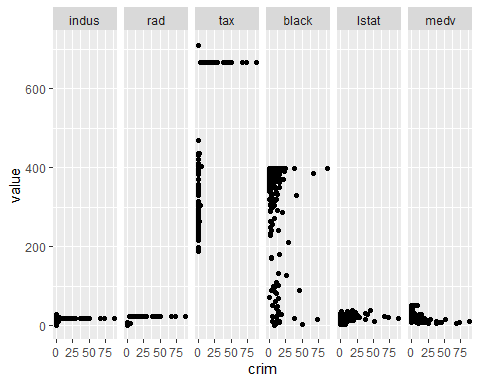
\includegraphics{STA_exam_ps33296_files/figure-latex/3.15.a-1.pdf}

\begin{Shaded}
\begin{Highlighting}[]
\CommentTok{\# These scatter plots show high variability wrt crim rate}
\end{Highlighting}
\end{Shaded}

\hypertarget{b-fit-a-multiple-regression-model-to-predict-the-response-using-all-of-the-predictors.-describe-your-results.-for-which-predictors-can-we-reject-the-null-hypothesis-h0-ux3b2j-0}{%
\paragraph{(b) Fit a multiple regression model to predict the response
using all of the predictors. Describe your results. For which predictors
can we reject the null hypothesis H0 : βj =
0?}\label{b-fit-a-multiple-regression-model-to-predict-the-response-using-all-of-the-predictors.-describe-your-results.-for-which-predictors-can-we-reject-the-null-hypothesis-h0-ux3b2j-0}}

\begin{Shaded}
\begin{Highlighting}[]
\NormalTok{lm\_fit }\OtherTok{=} \FunctionTok{lm}\NormalTok{(crim }\SpecialCharTok{\textasciitilde{}}\NormalTok{., }\AttributeTok{data=}\NormalTok{Boston) }

\NormalTok{lm\_fit\_tidy }\OtherTok{=} \FunctionTok{tidy}\NormalTok{(lm\_fit)}

\NormalTok{lm\_fit }\SpecialCharTok{\%\textgreater{}\%}\NormalTok{ summary}
\end{Highlighting}
\end{Shaded}

\begin{verbatim}
## 
## Call:
## lm(formula = crim ~ ., data = Boston)
## 
## Residuals:
##    Min     1Q Median     3Q    Max 
## -9.924 -2.120 -0.353  1.019 75.051 
## 
## Coefficients:
##               Estimate Std. Error t value Pr(>|t|)    
## (Intercept)  17.033228   7.234903   2.354 0.018949 *  
## zn            0.044855   0.018734   2.394 0.017025 *  
## indus        -0.063855   0.083407  -0.766 0.444294    
## chas         -0.749134   1.180147  -0.635 0.525867    
## nox         -10.313535   5.275536  -1.955 0.051152 .  
## rm            0.430131   0.612830   0.702 0.483089    
## age           0.001452   0.017925   0.081 0.935488    
## dis          -0.987176   0.281817  -3.503 0.000502 ***
## rad           0.588209   0.088049   6.680 6.46e-11 ***
## tax          -0.003780   0.005156  -0.733 0.463793    
## ptratio      -0.271081   0.186450  -1.454 0.146611    
## black        -0.007538   0.003673  -2.052 0.040702 *  
## lstat         0.126211   0.075725   1.667 0.096208 .  
## medv         -0.198887   0.060516  -3.287 0.001087 ** 
## ---
## Signif. codes:  0 '***' 0.001 '**' 0.01 '*' 0.05 '.' 0.1 ' ' 1
## 
## Residual standard error: 6.439 on 492 degrees of freedom
## Multiple R-squared:  0.454,  Adjusted R-squared:  0.4396 
## F-statistic: 31.47 on 13 and 492 DF,  p-value: < 2.2e-16
\end{verbatim}

We can reject the NULL hypothesis for zn, indus, dis, rad, black and
medv variables as they have a a significant p-value

\hypertarget{c-how-do-your-results-from-a-compare-to-your-results-from-b-create-a-plot-displaying-the-univariate-regression-coefficients-from-a-on-the-x-axis-and-the-multiple-regression-coefficients-from-b-on-the-y-axis.-that-is-each-predictor-is-displayed-as-a-single-point-in-the-plot.-its-coefficient-in-a-simple-linear-regression-model-is-shown-on-the-x-axis-and-its-coefficient-estimate-in-the-multiple-linear-regression-model-is-shown-on-the-y-axis.}{%
\paragraph{(c) How do your results from (a) compare to your results from
(b)? Create a plot displaying the univariate regression coefficients
from (a) on the x-axis, and the multiple regression coefficients from
(b) on the y-axis. That is, each predictor is displayed as a single
point in the plot. Its coefficient in a simple linear regression model
is shown on the x-axis, and its coefficient estimate in the multiple
linear regression model is shown on the
y-axis.}\label{c-how-do-your-results-from-a-compare-to-your-results-from-b-create-a-plot-displaying-the-univariate-regression-coefficients-from-a-on-the-x-axis-and-the-multiple-regression-coefficients-from-b-on-the-y-axis.-that-is-each-predictor-is-displayed-as-a-single-point-in-the-plot.-its-coefficient-in-a-simple-linear-regression-model-is-shown-on-the-x-axis-and-its-coefficient-estimate-in-the-multiple-linear-regression-model-is-shown-on-the-y-axis.}}

\begin{Shaded}
\begin{Highlighting}[]
\NormalTok{mutivariate\_reg\_betas }\OtherTok{=}\NormalTok{ lm\_fit\_tidy }\SpecialCharTok{\%\textgreater{}\%}\NormalTok{ dplyr}\SpecialCharTok{::}\FunctionTok{select}\NormalTok{(term, estimate) }\SpecialCharTok{\%\textgreater{}\%} 
  \FunctionTok{filter}\NormalTok{(term }\SpecialCharTok{!=} \StringTok{"(Intercept)"}\NormalTok{)}


\FunctionTok{plot}\NormalTok{(}\AttributeTok{x =}\NormalTok{ univariate\_reg\_betas}\SpecialCharTok{$}\NormalTok{estimate, }\AttributeTok{y =}\NormalTok{ mutivariate\_reg\_betas}\SpecialCharTok{$}\NormalTok{estimate)}
\FunctionTok{text}\NormalTok{(}\AttributeTok{x =}\NormalTok{ univariate\_reg\_betas}\SpecialCharTok{$}\NormalTok{estimate, }\AttributeTok{y =}\NormalTok{ mutivariate\_reg\_betas}\SpecialCharTok{$}\NormalTok{estimate, }\AttributeTok{labels =}\NormalTok{ univariate\_reg\_betas}\SpecialCharTok{$}\NormalTok{term, }\AttributeTok{pos=}\DecValTok{3}\NormalTok{)}
\end{Highlighting}
\end{Shaded}

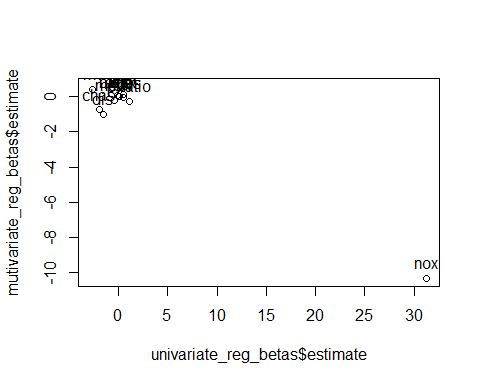
\includegraphics{STA_exam_ps33296_files/figure-latex/3.15.c-1.pdf}

nox is different in multivariate model compared to univariate. it is 31
in univariate and -10 in multivariate

\hypertarget{d-is-there-evidence-of-non-linear-association-between-any-of-the-predictors-and-the-response-to-answer-this-question-for-each-predictor-x-fit-a-model-of-the-form-y-ux3b20-ux3b21x-ux3b22x2-ux3b23x3-e.}{%
\paragraph{(d) Is there evidence of non-linear association between any
of the predictors and the response? To answer this question, for each
predictor X, fit a model of the form Y = β0 + β1X + β2X2 + β3X3 +
E.}\label{d-is-there-evidence-of-non-linear-association-between-any-of-the-predictors-and-the-response-to-answer-this-question-for-each-predictor-x-fit-a-model-of-the-form-y-ux3b20-ux3b21x-ux3b22x2-ux3b23x3-e.}}

\begin{Shaded}
\begin{Highlighting}[]
\NormalTok{predictorlist }\OtherTok{=} \FunctionTok{colnames}\NormalTok{(Boston }\SpecialCharTok{\%\textgreater{}\%}\NormalTok{ dplyr}\SpecialCharTok{::}\FunctionTok{select}\NormalTok{(}\SpecialCharTok{{-}}\NormalTok{crim))}

\NormalTok{univariate\_poly\_reg\_betas }\OtherTok{=} \FunctionTok{data.frame}\NormalTok{()}
\NormalTok{k }\OtherTok{=} \DecValTok{1}
\ControlFlowTok{for}\NormalTok{ (i }\ControlFlowTok{in}\NormalTok{ predictorlist)\{ }
  \FunctionTok{print}\NormalTok{(i)}
\NormalTok{  fit }\OtherTok{=} \FunctionTok{lm}\NormalTok{(}\FunctionTok{paste}\NormalTok{(}\StringTok{"crim \textasciitilde{}"}\NormalTok{, i[[}\DecValTok{1}\NormalTok{]], }\StringTok{"+ I("}\NormalTok{,i[[}\DecValTok{1}\NormalTok{]],}\StringTok{"\^{}2) + I("}\NormalTok{,i[[}\DecValTok{1}\NormalTok{]],}\StringTok{"\^{}3)"}\NormalTok{), }\AttributeTok{data=}\NormalTok{Boston) }
  \CommentTok{\# summary\_stat = tidy(fit)}
  \FunctionTok{print}\NormalTok{(}\FunctionTok{summary}\NormalTok{(fit))}
\NormalTok{  summary\_stat }\OtherTok{=}\NormalTok{ summary\_stat }\SpecialCharTok{\%\textgreater{}\%}\NormalTok{ dplyr}\SpecialCharTok{::}\FunctionTok{select}\NormalTok{(term, estimate) }\SpecialCharTok{\%\textgreater{}\%} \FunctionTok{filter}\NormalTok{(term }\SpecialCharTok{==}\NormalTok{ i)}
\NormalTok{  univariate\_poly\_reg\_betas }\OtherTok{=} \FunctionTok{rbind}\NormalTok{(univariate\_poly\_reg\_betas, summary\_stat)}
\NormalTok{\} }
\end{Highlighting}
\end{Shaded}

\begin{verbatim}
## [1] "zn"
## 
## Call:
## lm(formula = paste("crim ~", i[[1]], "+ I(", i[[1]], "^2) + I(", 
##     i[[1]], "^3)"), data = Boston)
## 
## Residuals:
##    Min     1Q Median     3Q    Max 
## -4.821 -4.614 -1.294  0.473 84.130 
## 
## Coefficients:
##               Estimate Std. Error t value Pr(>|t|)    
## (Intercept)  4.846e+00  4.330e-01  11.192  < 2e-16 ***
## zn          -3.322e-01  1.098e-01  -3.025  0.00261 ** 
## I(zn^2)      6.483e-03  3.861e-03   1.679  0.09375 .  
## I(zn^3)     -3.776e-05  3.139e-05  -1.203  0.22954    
## ---
## Signif. codes:  0 '***' 0.001 '**' 0.01 '*' 0.05 '.' 0.1 ' ' 1
## 
## Residual standard error: 8.372 on 502 degrees of freedom
## Multiple R-squared:  0.05824,    Adjusted R-squared:  0.05261 
## F-statistic: 10.35 on 3 and 502 DF,  p-value: 1.281e-06
## 
## [1] "indus"
## 
## Call:
## lm(formula = paste("crim ~", i[[1]], "+ I(", i[[1]], "^2) + I(", 
##     i[[1]], "^3)"), data = Boston)
## 
## Residuals:
##    Min     1Q Median     3Q    Max 
## -8.278 -2.514  0.054  0.764 79.713 
## 
## Coefficients:
##               Estimate Std. Error t value Pr(>|t|)    
## (Intercept)  3.6625683  1.5739833   2.327   0.0204 *  
## indus       -1.9652129  0.4819901  -4.077 5.30e-05 ***
## I(indus^2)   0.2519373  0.0393221   6.407 3.42e-10 ***
## I(indus^3)  -0.0069760  0.0009567  -7.292 1.20e-12 ***
## ---
## Signif. codes:  0 '***' 0.001 '**' 0.01 '*' 0.05 '.' 0.1 ' ' 1
## 
## Residual standard error: 7.423 on 502 degrees of freedom
## Multiple R-squared:  0.2597, Adjusted R-squared:  0.2552 
## F-statistic: 58.69 on 3 and 502 DF,  p-value: < 2.2e-16
## 
## [1] "chas"
## 
## Call:
## lm(formula = paste("crim ~", i[[1]], "+ I(", i[[1]], "^2) + I(", 
##     i[[1]], "^3)"), data = Boston)
## 
## Residuals:
##    Min     1Q Median     3Q    Max 
## -3.738 -3.661 -3.435  0.018 85.232 
## 
## Coefficients: (2 not defined because of singularities)
##             Estimate Std. Error t value Pr(>|t|)    
## (Intercept)   3.7444     0.3961   9.453   <2e-16 ***
## chas         -1.8928     1.5061  -1.257    0.209    
## I(chas^2)         NA         NA      NA       NA    
## I(chas^3)         NA         NA      NA       NA    
## ---
## Signif. codes:  0 '***' 0.001 '**' 0.01 '*' 0.05 '.' 0.1 ' ' 1
## 
## Residual standard error: 8.597 on 504 degrees of freedom
## Multiple R-squared:  0.003124,   Adjusted R-squared:  0.001146 
## F-statistic: 1.579 on 1 and 504 DF,  p-value: 0.2094
## 
## [1] "nox"
## 
## Call:
## lm(formula = paste("crim ~", i[[1]], "+ I(", i[[1]], "^2) + I(", 
##     i[[1]], "^3)"), data = Boston)
## 
## Residuals:
##    Min     1Q Median     3Q    Max 
## -9.110 -2.068 -0.255  0.739 78.302 
## 
## Coefficients:
##             Estimate Std. Error t value Pr(>|t|)    
## (Intercept)   233.09      33.64   6.928 1.31e-11 ***
## nox         -1279.37     170.40  -7.508 2.76e-13 ***
## I(nox^2)     2248.54     279.90   8.033 6.81e-15 ***
## I(nox^3)    -1245.70     149.28  -8.345 6.96e-16 ***
## ---
## Signif. codes:  0 '***' 0.001 '**' 0.01 '*' 0.05 '.' 0.1 ' ' 1
## 
## Residual standard error: 7.234 on 502 degrees of freedom
## Multiple R-squared:  0.297,  Adjusted R-squared:  0.2928 
## F-statistic: 70.69 on 3 and 502 DF,  p-value: < 2.2e-16
## 
## [1] "rm"
## 
## Call:
## lm(formula = paste("crim ~", i[[1]], "+ I(", i[[1]], "^2) + I(", 
##     i[[1]], "^3)"), data = Boston)
## 
## Residuals:
##     Min      1Q  Median      3Q     Max 
## -18.485  -3.468  -2.221  -0.015  87.219 
## 
## Coefficients:
##             Estimate Std. Error t value Pr(>|t|)  
## (Intercept) 112.6246    64.5172   1.746   0.0815 .
## rm          -39.1501    31.3115  -1.250   0.2118  
## I(rm^2)       4.5509     5.0099   0.908   0.3641  
## I(rm^3)      -0.1745     0.2637  -0.662   0.5086  
## ---
## Signif. codes:  0 '***' 0.001 '**' 0.01 '*' 0.05 '.' 0.1 ' ' 1
## 
## Residual standard error: 8.33 on 502 degrees of freedom
## Multiple R-squared:  0.06779,    Adjusted R-squared:  0.06222 
## F-statistic: 12.17 on 3 and 502 DF,  p-value: 1.067e-07
## 
## [1] "age"
## 
## Call:
## lm(formula = paste("crim ~", i[[1]], "+ I(", i[[1]], "^2) + I(", 
##     i[[1]], "^3)"), data = Boston)
## 
## Residuals:
##    Min     1Q Median     3Q    Max 
## -9.762 -2.673 -0.516  0.019 82.842 
## 
## Coefficients:
##               Estimate Std. Error t value Pr(>|t|)   
## (Intercept) -2.549e+00  2.769e+00  -0.920  0.35780   
## age          2.737e-01  1.864e-01   1.468  0.14266   
## I(age^2)    -7.230e-03  3.637e-03  -1.988  0.04738 * 
## I(age^3)     5.745e-05  2.109e-05   2.724  0.00668 **
## ---
## Signif. codes:  0 '***' 0.001 '**' 0.01 '*' 0.05 '.' 0.1 ' ' 1
## 
## Residual standard error: 7.84 on 502 degrees of freedom
## Multiple R-squared:  0.1742, Adjusted R-squared:  0.1693 
## F-statistic: 35.31 on 3 and 502 DF,  p-value: < 2.2e-16
## 
## [1] "dis"
## 
## Call:
## lm(formula = paste("crim ~", i[[1]], "+ I(", i[[1]], "^2) + I(", 
##     i[[1]], "^3)"), data = Boston)
## 
## Residuals:
##     Min      1Q  Median      3Q     Max 
## -10.757  -2.588   0.031   1.267  76.378 
## 
## Coefficients:
##             Estimate Std. Error t value Pr(>|t|)    
## (Intercept)  30.0476     2.4459  12.285  < 2e-16 ***
## dis         -15.5543     1.7360  -8.960  < 2e-16 ***
## I(dis^2)      2.4521     0.3464   7.078 4.94e-12 ***
## I(dis^3)     -0.1186     0.0204  -5.814 1.09e-08 ***
## ---
## Signif. codes:  0 '***' 0.001 '**' 0.01 '*' 0.05 '.' 0.1 ' ' 1
## 
## Residual standard error: 7.331 on 502 degrees of freedom
## Multiple R-squared:  0.2778, Adjusted R-squared:  0.2735 
## F-statistic: 64.37 on 3 and 502 DF,  p-value: < 2.2e-16
## 
## [1] "rad"
## 
## Call:
## lm(formula = paste("crim ~", i[[1]], "+ I(", i[[1]], "^2) + I(", 
##     i[[1]], "^3)"), data = Boston)
## 
## Residuals:
##     Min      1Q  Median      3Q     Max 
## -10.381  -0.412  -0.269   0.179  76.217 
## 
## Coefficients:
##              Estimate Std. Error t value Pr(>|t|)
## (Intercept) -0.605545   2.050108  -0.295    0.768
## rad          0.512736   1.043597   0.491    0.623
## I(rad^2)    -0.075177   0.148543  -0.506    0.613
## I(rad^3)     0.003209   0.004564   0.703    0.482
## 
## Residual standard error: 6.682 on 502 degrees of freedom
## Multiple R-squared:    0.4,  Adjusted R-squared:  0.3965 
## F-statistic: 111.6 on 3 and 502 DF,  p-value: < 2.2e-16
## 
## [1] "tax"
## 
## Call:
## lm(formula = paste("crim ~", i[[1]], "+ I(", i[[1]], "^2) + I(", 
##     i[[1]], "^3)"), data = Boston)
## 
## Residuals:
##     Min      1Q  Median      3Q     Max 
## -13.273  -1.389   0.046   0.536  76.950 
## 
## Coefficients:
##               Estimate Std. Error t value Pr(>|t|)
## (Intercept)  1.918e+01  1.180e+01   1.626    0.105
## tax         -1.533e-01  9.568e-02  -1.602    0.110
## I(tax^2)     3.608e-04  2.425e-04   1.488    0.137
## I(tax^3)    -2.204e-07  1.889e-07  -1.167    0.244
## 
## Residual standard error: 6.854 on 502 degrees of freedom
## Multiple R-squared:  0.3689, Adjusted R-squared:  0.3651 
## F-statistic:  97.8 on 3 and 502 DF,  p-value: < 2.2e-16
## 
## [1] "ptratio"
## 
## Call:
## lm(formula = paste("crim ~", i[[1]], "+ I(", i[[1]], "^2) + I(", 
##     i[[1]], "^3)"), data = Boston)
## 
## Residuals:
##    Min     1Q Median     3Q    Max 
## -6.833 -4.146 -1.655  1.408 82.697 
## 
## Coefficients:
##               Estimate Std. Error t value Pr(>|t|)   
## (Intercept)  477.18405  156.79498   3.043  0.00246 **
## ptratio      -82.36054   27.64394  -2.979  0.00303 **
## I(ptratio^2)   4.63535    1.60832   2.882  0.00412 **
## I(ptratio^3)  -0.08476    0.03090  -2.743  0.00630 **
## ---
## Signif. codes:  0 '***' 0.001 '**' 0.01 '*' 0.05 '.' 0.1 ' ' 1
## 
## Residual standard error: 8.122 on 502 degrees of freedom
## Multiple R-squared:  0.1138, Adjusted R-squared:  0.1085 
## F-statistic: 21.48 on 3 and 502 DF,  p-value: 4.171e-13
## 
## [1] "black"
## 
## Call:
## lm(formula = paste("crim ~", i[[1]], "+ I(", i[[1]], "^2) + I(", 
##     i[[1]], "^3)"), data = Boston)
## 
## Residuals:
##     Min      1Q  Median      3Q     Max 
## -13.096  -2.343  -2.128  -1.439  86.790 
## 
## Coefficients:
##               Estimate Std. Error t value Pr(>|t|)    
## (Intercept)  1.826e+01  2.305e+00   7.924  1.5e-14 ***
## black       -8.356e-02  5.633e-02  -1.483    0.139    
## I(black^2)   2.137e-04  2.984e-04   0.716    0.474    
## I(black^3)  -2.652e-07  4.364e-07  -0.608    0.544    
## ---
## Signif. codes:  0 '***' 0.001 '**' 0.01 '*' 0.05 '.' 0.1 ' ' 1
## 
## Residual standard error: 7.955 on 502 degrees of freedom
## Multiple R-squared:  0.1498, Adjusted R-squared:  0.1448 
## F-statistic: 29.49 on 3 and 502 DF,  p-value: < 2.2e-16
## 
## [1] "lstat"
## 
## Call:
## lm(formula = paste("crim ~", i[[1]], "+ I(", i[[1]], "^2) + I(", 
##     i[[1]], "^3)"), data = Boston)
## 
## Residuals:
##     Min      1Q  Median      3Q     Max 
## -15.234  -2.151  -0.486   0.066  83.353 
## 
## Coefficients:
##               Estimate Std. Error t value Pr(>|t|)  
## (Intercept)  1.2009656  2.0286452   0.592   0.5541  
## lstat       -0.4490656  0.4648911  -0.966   0.3345  
## I(lstat^2)   0.0557794  0.0301156   1.852   0.0646 .
## I(lstat^3)  -0.0008574  0.0005652  -1.517   0.1299  
## ---
## Signif. codes:  0 '***' 0.001 '**' 0.01 '*' 0.05 '.' 0.1 ' ' 1
## 
## Residual standard error: 7.629 on 502 degrees of freedom
## Multiple R-squared:  0.2179, Adjusted R-squared:  0.2133 
## F-statistic: 46.63 on 3 and 502 DF,  p-value: < 2.2e-16
## 
## [1] "medv"
## 
## Call:
## lm(formula = paste("crim ~", i[[1]], "+ I(", i[[1]], "^2) + I(", 
##     i[[1]], "^3)"), data = Boston)
## 
## Residuals:
##     Min      1Q  Median      3Q     Max 
## -24.427  -1.976  -0.437   0.439  73.655 
## 
## Coefficients:
##               Estimate Std. Error t value Pr(>|t|)    
## (Intercept) 53.1655381  3.3563105  15.840  < 2e-16 ***
## medv        -5.0948305  0.4338321 -11.744  < 2e-16 ***
## I(medv^2)    0.1554965  0.0171904   9.046  < 2e-16 ***
## I(medv^3)   -0.0014901  0.0002038  -7.312 1.05e-12 ***
## ---
## Signif. codes:  0 '***' 0.001 '**' 0.01 '*' 0.05 '.' 0.1 ' ' 1
## 
## Residual standard error: 6.569 on 502 degrees of freedom
## Multiple R-squared:  0.4202, Adjusted R-squared:  0.4167 
## F-statistic: 121.3 on 3 and 502 DF,  p-value: < 2.2e-16
\end{verbatim}

\begin{itemize}
\item
  zn, Indus, Indus\^{}2, Indus\^{}3, nox, nox\^{}2, nox\^{}3, age\^{}2,
  age\^{}3, dis, dis\^{}2, dis\^{}3, ptratio, ptratio\^{}2,
  ptratio\^{}3, medv, medv\^{}2, medv\^{}3 are statistically
  significant.
\item
  chas, rm, rad, tax and their polynomial terms are not significant at
  all, and none of its polynomial terms are significant
\end{itemize}

\begin{center}\rule{0.5\linewidth}{0.5pt}\end{center}

\hypertarget{chapter-6}{%
\section{Chapter 6}\label{chapter-6}}

\hypertarget{question-9}{%
\subsubsection{Question 9}\label{question-9}}

In this exercise, we will predict the number of applications received
using the other variables in the College data set.

\hypertarget{a-split-the-data-set-into-a-training-set-and-a-test-set.}{%
\paragraph{(a) Split the data set into a training set and a test
set.}\label{a-split-the-data-set-into-a-training-set-and-a-test-set.}}

\begin{Shaded}
\begin{Highlighting}[]
\FunctionTok{rm}\NormalTok{(}\AttributeTok{list =} \FunctionTok{ls}\NormalTok{())}
\FunctionTok{library}\NormalTok{(ISLR)}
\FunctionTok{library}\NormalTok{(tidyverse)}
\FunctionTok{library}\NormalTok{(glmnet)}
\FunctionTok{library}\NormalTok{(pls)}

\NormalTok{college\_dat }\OtherTok{=}\NormalTok{ College}

\CommentTok{\# splitting dataset with 70:30 split (train{-}test)}
\NormalTok{n }\OtherTok{=}\NormalTok{ college\_dat }\SpecialCharTok{\%\textgreater{}\%}\NormalTok{ nrow}
\NormalTok{idx }\OtherTok{=} \FunctionTok{sample}\NormalTok{(}\DecValTok{1}\SpecialCharTok{:}\NormalTok{n, }\FloatTok{0.7}\SpecialCharTok{*}\NormalTok{n)}


\NormalTok{train }\OtherTok{=}\NormalTok{ college\_dat[idx,]}
\CommentTok{\# length of training set}
\FunctionTok{nrow}\NormalTok{(train)}
\end{Highlighting}
\end{Shaded}

\begin{verbatim}
## [1] 543
\end{verbatim}

\begin{Shaded}
\begin{Highlighting}[]
\NormalTok{test }\OtherTok{=}\NormalTok{ college\_dat[}\SpecialCharTok{{-}}\NormalTok{idx,]}
\CommentTok{\# length of testing set}
\FunctionTok{nrow}\NormalTok{(test)}
\end{Highlighting}
\end{Shaded}

\begin{verbatim}
## [1] 234
\end{verbatim}

\hypertarget{b-fit-a-linear-model-using-least-squares-on-the-training-set-and-report-the-test-error-obtained.}{%
\paragraph{(b) Fit a linear model using least squares on the training
set, and report the test error
obtained.}\label{b-fit-a-linear-model-using-least-squares-on-the-training-set-and-report-the-test-error-obtained.}}

\begin{Shaded}
\begin{Highlighting}[]
\NormalTok{lm\_fit }\OtherTok{=} \FunctionTok{lm}\NormalTok{(Apps}\SpecialCharTok{\textasciitilde{}}\NormalTok{., }\AttributeTok{data =}\NormalTok{ train)}


\NormalTok{prediction }\OtherTok{=} \FunctionTok{predict}\NormalTok{(lm\_fit, test}\SpecialCharTok{\%\textgreater{}\%}\NormalTok{ dplyr}\SpecialCharTok{::}\FunctionTok{select}\NormalTok{(}\SpecialCharTok{{-}}\NormalTok{Apps))}

\CommentTok{\# MSE Error in lm fit}
\NormalTok{MSE\_lm }\OtherTok{=} \FunctionTok{mean}\NormalTok{((test[, }\StringTok{"Apps"}\NormalTok{] }\SpecialCharTok{{-}}\NormalTok{ prediction)}\SpecialCharTok{\^{}}\DecValTok{2}\NormalTok{)}
\NormalTok{MSE\_lm}
\end{Highlighting}
\end{Shaded}

\begin{verbatim}
## [1] 944997
\end{verbatim}

\hypertarget{c-fit-a-ridge-regression-model-on-the-training-set-with-ux3bb-chosen-by-cross-validation.-report-the-test-error-obtained}{%
\paragraph{(c) Fit a ridge regression model on the training set, with λ
chosen by cross-validation. Report the test error
obtained}\label{c-fit-a-ridge-regression-model-on-the-training-set-with-ux3bb-chosen-by-cross-validation.-report-the-test-error-obtained}}

\begin{Shaded}
\begin{Highlighting}[]
\NormalTok{train\_mat }\OtherTok{=} \FunctionTok{model.matrix}\NormalTok{(Apps}\SpecialCharTok{\textasciitilde{}}\NormalTok{., }\AttributeTok{data=}\NormalTok{train)}
\NormalTok{test\_mat }\OtherTok{=} \FunctionTok{model.matrix}\NormalTok{(Apps}\SpecialCharTok{\textasciitilde{}}\NormalTok{., }\AttributeTok{data=}\NormalTok{test)}
\NormalTok{grid }\OtherTok{=} \DecValTok{10} \SpecialCharTok{\^{}} \FunctionTok{seq}\NormalTok{(}\DecValTok{4}\NormalTok{, }\SpecialCharTok{{-}}\DecValTok{2}\NormalTok{, }\AttributeTok{length=}\DecValTok{100}\NormalTok{)}

\NormalTok{ridge\_model }\OtherTok{=} \FunctionTok{cv.glmnet}\NormalTok{(train\_mat, train[,}\StringTok{"Apps"}\NormalTok{], }\AttributeTok{alpha=}\DecValTok{0}\NormalTok{, }\AttributeTok{lambda=}\NormalTok{grid)}
\NormalTok{lambda\_best }\OtherTok{=}\NormalTok{ ridge\_model}\SpecialCharTok{$}\NormalTok{lambda.min}
\NormalTok{lambda\_best}
\end{Highlighting}
\end{Shaded}

\begin{verbatim}
## [1] 0.01
\end{verbatim}

\begin{Shaded}
\begin{Highlighting}[]
\NormalTok{ridge\_prediction }\OtherTok{=} \FunctionTok{predict}\NormalTok{(ridge\_model, }\AttributeTok{newx=}\NormalTok{test\_mat, }\AttributeTok{s=}\NormalTok{lambda\_best)}
\NormalTok{MSE\_ridge }\OtherTok{=} \FunctionTok{mean}\NormalTok{((test[, }\StringTok{"Apps"}\NormalTok{] }\SpecialCharTok{{-}}\NormalTok{ ridge\_prediction)}\SpecialCharTok{\^{}}\DecValTok{2}\NormalTok{)}

\FunctionTok{cat}\NormalTok{(MSE\_ridge)}
\end{Highlighting}
\end{Shaded}

\begin{verbatim}
## 944943.1
\end{verbatim}

\hypertarget{d-fit-a-lasso-model-on-the-training-set-with-ux3bb-chosen-by-cross-validation.-report-the-test-error-obtained}{%
\paragraph{(d) Fit a lasso model on the training set, with λ chosen by
cross-validation. Report the test error
obtained}\label{d-fit-a-lasso-model-on-the-training-set-with-ux3bb-chosen-by-cross-validation.-report-the-test-error-obtained}}

\begin{Shaded}
\begin{Highlighting}[]
\NormalTok{lasso\_model }\OtherTok{=} \FunctionTok{cv.glmnet}\NormalTok{(train\_mat, train[,}\StringTok{"Apps"}\NormalTok{], }\AttributeTok{alpha=}\DecValTok{1}\NormalTok{, }\AttributeTok{lambda=}\NormalTok{grid)}
\NormalTok{lambda\_best }\OtherTok{=}\NormalTok{ lasso\_model}\SpecialCharTok{$}\NormalTok{lambda.min}
\NormalTok{lambda\_best}
\end{Highlighting}
\end{Shaded}

\begin{verbatim}
## [1] 16.29751
\end{verbatim}

\begin{Shaded}
\begin{Highlighting}[]
\NormalTok{lasso\_prediction }\OtherTok{=} \FunctionTok{predict}\NormalTok{(lasso\_model, }\AttributeTok{newx=}\NormalTok{test\_mat, }\AttributeTok{s=}\NormalTok{lambda\_best)}

\NormalTok{MSE\_lasso }\OtherTok{=} \FunctionTok{mean}\NormalTok{((test[, }\StringTok{"Apps"}\NormalTok{] }\SpecialCharTok{{-}}\NormalTok{ lasso\_prediction)}\SpecialCharTok{\^{}}\DecValTok{2}\NormalTok{)}

\FunctionTok{predict}\NormalTok{(lasso\_model, }\AttributeTok{s=}\NormalTok{lambda\_best, }\AttributeTok{type=}\StringTok{"coefficients"}\NormalTok{)}
\end{Highlighting}
\end{Shaded}

\begin{verbatim}
## 19 x 1 sparse Matrix of class "dgCMatrix"
##                        s1
## (Intercept) -5.837606e+02
## (Intercept)  .           
## PrivateYes  -4.269256e+02
## Accept       1.529231e+00
## Enroll      -3.788805e-01
## Top10perc    5.362316e+01
## Top25perc   -1.556098e+01
## F.Undergrad  .           
## P.Undergrad  1.135483e-02
## Outstate    -8.684699e-02
## Room.Board   1.463687e-01
## Books        8.981397e-03
## Personal     .           
## PhD         -6.905472e+00
## Terminal    -2.378792e+00
## S.F.Ratio    1.675980e+01
## perc.alumni  .           
## Expend       7.895846e-02
## Grad.Rate    7.261171e+00
\end{verbatim}

\begin{Shaded}
\begin{Highlighting}[]
\FunctionTok{cat}\NormalTok{(MSE\_lasso)}
\end{Highlighting}
\end{Shaded}

\begin{verbatim}
## 870311
\end{verbatim}

\hypertarget{e-fit-a-pcr-model-on-the-training-set-with-m-chosen-by-crossvalidation.-report-the-test-error-obtained-along-with-the-value-of-m-selected-by-cross-validation.}{%
\paragraph{(e) Fit a PCR model on the training set, with M chosen by
crossvalidation. Report the test error obtained, along with the value of
M selected by
cross-validation.}\label{e-fit-a-pcr-model-on-the-training-set-with-m-chosen-by-crossvalidation.-report-the-test-error-obtained-along-with-the-value-of-m-selected-by-cross-validation.}}

\begin{Shaded}
\begin{Highlighting}[]
\NormalTok{pcr\_fit }\OtherTok{=} \FunctionTok{pcr}\NormalTok{(Apps}\SpecialCharTok{\textasciitilde{}}\NormalTok{., }\AttributeTok{data=}\NormalTok{train, }\AttributeTok{scale=}\NormalTok{T, }\AttributeTok{validation=}\StringTok{"CV"}\NormalTok{)}

\FunctionTok{cat}\NormalTok{(}\FunctionTok{validationplot}\NormalTok{(pcr\_fit, }\AttributeTok{val\_type=}\StringTok{"MSEP"}\NormalTok{))}
\end{Highlighting}
\end{Shaded}

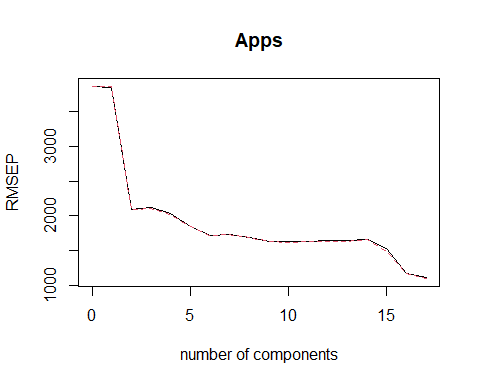
\includegraphics{STA_exam_ps33296_files/figure-latex/6.9.e-1.pdf}

\begin{Shaded}
\begin{Highlighting}[]
\NormalTok{pcr\_pred }\OtherTok{=} \FunctionTok{predict}\NormalTok{(pcr\_fit, test, }\AttributeTok{ncomp=}\DecValTok{8}\NormalTok{)}

\NormalTok{MSE\_pcr }\OtherTok{=}\NormalTok{ (}\FunctionTok{mean}\NormalTok{((test[, }\StringTok{"Apps"}\NormalTok{] }\SpecialCharTok{{-}}\NormalTok{ pcr\_pred)}\SpecialCharTok{\^{}}\DecValTok{2}\NormalTok{))}
\FunctionTok{cat}\NormalTok{(MSE\_pcr)}
\end{Highlighting}
\end{Shaded}

\begin{verbatim}
## 1654239
\end{verbatim}

\hypertarget{f-fit-a-pls-model-on-the-training-set-with-m-chosen-by-crossvalidation.-report-the-test-error-obtained-along-with-the-value-of-m-selected-by-cross-validation}{%
\paragraph{(f) Fit a PLS model on the training set, with M chosen by
crossvalidation. Report the test error obtained, along with the value of
M selected by
cross-validation}\label{f-fit-a-pls-model-on-the-training-set-with-m-chosen-by-crossvalidation.-report-the-test-error-obtained-along-with-the-value-of-m-selected-by-cross-validation}}

\begin{Shaded}
\begin{Highlighting}[]
\NormalTok{pls\_fit }\OtherTok{=} \FunctionTok{plsr}\NormalTok{(Apps}\SpecialCharTok{\textasciitilde{}}\NormalTok{., }\AttributeTok{data=}\NormalTok{train, }\AttributeTok{scale=}\NormalTok{T, }\AttributeTok{validation=}\StringTok{"CV"}\NormalTok{)}

\FunctionTok{cat}\NormalTok{(}\FunctionTok{validationplot}\NormalTok{(pls\_fit, }\AttributeTok{val\_type=}\StringTok{"MSEP"}\NormalTok{))}
\end{Highlighting}
\end{Shaded}

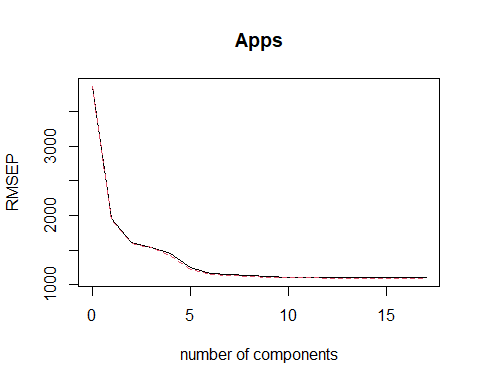
\includegraphics{STA_exam_ps33296_files/figure-latex/6.9.f-1.pdf}

\begin{Shaded}
\begin{Highlighting}[]
\NormalTok{pls\_pred }\OtherTok{=} \FunctionTok{predict}\NormalTok{(pls\_fit, test, }\AttributeTok{ncomp=}\DecValTok{8}\NormalTok{)}

\NormalTok{MSE\_pls }\OtherTok{=} \FunctionTok{mean}\NormalTok{((test[, }\StringTok{"Apps"}\NormalTok{] }\SpecialCharTok{{-}}\NormalTok{ pls\_pred)}\SpecialCharTok{\^{}}\DecValTok{2}\NormalTok{)}
\FunctionTok{cat}\NormalTok{(MSE\_pls)}
\end{Highlighting}
\end{Shaded}

\begin{verbatim}
## 954047.7
\end{verbatim}

\hypertarget{g-comment-on-the-results-obtained.-how-accurately-can-we-predict-the-number-of-college-applications-received-is-there-much-difference-among-the-test-errors-resulting-from-these-five-approaches}{%
\paragraph{(g) Comment on the results obtained. How accurately can we
predict the number of college applications received? Is there much
difference among the test errors resulting from these five
approaches?}\label{g-comment-on-the-results-obtained.-how-accurately-can-we-predict-the-number-of-college-applications-received-is-there-much-difference-among-the-test-errors-resulting-from-these-five-approaches}}

Except for PCR, all other predictors are able to predict the
Applications pretty accurately

\begin{Shaded}
\begin{Highlighting}[]
\NormalTok{avg }\OtherTok{=} \FunctionTok{mean}\NormalTok{(test[, }\StringTok{"Apps"}\NormalTok{])}
\NormalTok{mean\_variance }\OtherTok{=} \FunctionTok{mean}\NormalTok{((test[, }\StringTok{"Apps"}\NormalTok{] }\SpecialCharTok{{-}}\NormalTok{ avg)}\SpecialCharTok{\^{}}\DecValTok{2}\NormalTok{)}

\NormalTok{lm\_r2 }\OtherTok{=} \DecValTok{1} \SpecialCharTok{{-}}\NormalTok{ (MSE\_lm }\SpecialCharTok{/}\NormalTok{mean\_variance)}
\NormalTok{ridge\_r2 }\OtherTok{=} \DecValTok{1} \SpecialCharTok{{-}}\NormalTok{ (MSE\_ridge}\SpecialCharTok{/}\NormalTok{mean\_variance)}
\NormalTok{lasso\_r2 }\OtherTok{=} \DecValTok{1} \SpecialCharTok{{-}}\NormalTok{ (MSE\_lasso}\SpecialCharTok{/}\NormalTok{mean\_variance)}
\NormalTok{pcr\_r2 }\OtherTok{=} \DecValTok{1} \SpecialCharTok{{-}}\NormalTok{ (MSE\_pcr}\SpecialCharTok{/}\NormalTok{mean\_variance)}
\NormalTok{pls\_r2 }\OtherTok{=} \DecValTok{1} \SpecialCharTok{{-}}\NormalTok{ (MSE\_pls}\SpecialCharTok{/}\NormalTok{mean\_variance)}
\FunctionTok{barplot}\NormalTok{(}\FunctionTok{c}\NormalTok{(lm\_r2, ridge\_r2, lasso\_r2, pcr\_r2, pls\_r2), }\AttributeTok{names.arg=}\FunctionTok{c}\NormalTok{(}\StringTok{"OLS"}\NormalTok{, }\StringTok{"Ridge"}\NormalTok{, }\StringTok{"Lasso"}\NormalTok{, }\StringTok{"PCR"}\NormalTok{, }\StringTok{"PLS"}\NormalTok{), }\AttributeTok{main=}\StringTok{"Test R{-}squared"}\NormalTok{)}
\end{Highlighting}
\end{Shaded}

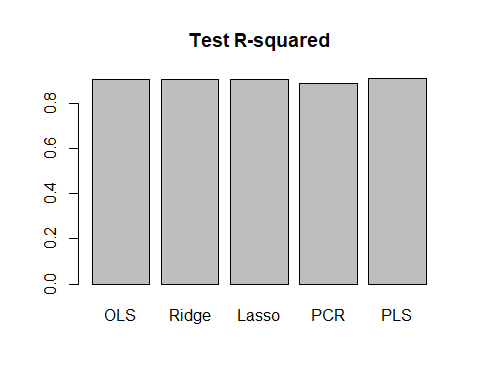
\includegraphics{STA_exam_ps33296_files/figure-latex/6.9.g-1.pdf}

\begin{center}\rule{0.5\linewidth}{0.5pt}\end{center}

\hypertarget{chapter-6-1}{%
\section{Chapter 6}\label{chapter-6-1}}

\hypertarget{question-11}{%
\subsubsection{Question 11}\label{question-11}}

In this exercise, we will predict the number of applications received
using the other variables in the College data set.

\hypertarget{a-try-out-some-of-the-regression-methods-explored-in-this-chapter-such-as-best-subset-selection-the-lasso-ridge-regression-and-pcr.-present-and-discuss-results-for-the-approaches-that-you-consider.}{%
\paragraph{(a) Try out some of the regression methods explored in this
chapter, such as best subset selection, the lasso, ridge regression, and
PCR. Present and discuss results for the approaches that you
consider.}\label{a-try-out-some-of-the-regression-methods-explored-in-this-chapter-such-as-best-subset-selection-the-lasso-ridge-regression-and-pcr.-present-and-discuss-results-for-the-approaches-that-you-consider.}}

\begin{Shaded}
\begin{Highlighting}[]
\FunctionTok{rm}\NormalTok{(}\AttributeTok{list =} \FunctionTok{ls}\NormalTok{())}
\FunctionTok{library}\NormalTok{(MASS)}
\FunctionTok{library}\NormalTok{(tidyverse)}
\FunctionTok{library}\NormalTok{(glmnet)}
\FunctionTok{library}\NormalTok{(pls)}
\FunctionTok{library}\NormalTok{(boot)}

\NormalTok{boston\_dat }\OtherTok{=}\NormalTok{ Boston}

\FunctionTok{set.seed}\NormalTok{(}\DecValTok{123}\NormalTok{)}
\CommentTok{\# splitting dataset with 70:30 split (train{-}test)}
\NormalTok{n }\OtherTok{=}\NormalTok{ boston\_dat }\SpecialCharTok{\%\textgreater{}\%}\NormalTok{ nrow}
\NormalTok{idx }\OtherTok{=} \FunctionTok{sample}\NormalTok{(}\DecValTok{1}\SpecialCharTok{:}\NormalTok{n, }\FloatTok{0.7}\SpecialCharTok{*}\NormalTok{n)}


\NormalTok{dfTraining }\OtherTok{=}\NormalTok{ boston\_dat[idx,]}
\CommentTok{\# length of training set}
\FunctionTok{nrow}\NormalTok{(dfTraining)}
\end{Highlighting}
\end{Shaded}

\begin{verbatim}
## [1] 354
\end{verbatim}

\begin{Shaded}
\begin{Highlighting}[]
\NormalTok{dfTest }\OtherTok{=}\NormalTok{ boston\_dat[}\SpecialCharTok{{-}}\NormalTok{idx,]}
\CommentTok{\# length of testing set}
\FunctionTok{nrow}\NormalTok{(dfTest)}
\end{Highlighting}
\end{Shaded}

\begin{verbatim}
## [1] 152
\end{verbatim}

\begin{Shaded}
\begin{Highlighting}[]
\DocumentationTok{\#\# a. subset selection  \#\#\#\#\#\#\#\#\#\#\#\#\#\#\#\#\#}
\NormalTok{deltas\_lm }\OtherTok{=} \FunctionTok{data.frame}\NormalTok{(}\AttributeTok{delta1=}\DecValTok{0}\NormalTok{, }\AttributeTok{delta2=}\DecValTok{0}\NormalTok{)}
\ControlFlowTok{for}\NormalTok{ (i }\ControlFlowTok{in} \DecValTok{1}\SpecialCharTok{:}\DecValTok{5}\NormalTok{)\{}
\NormalTok{ lm\_fit }\OtherTok{=} \FunctionTok{glm}\NormalTok{(crim}\SpecialCharTok{\textasciitilde{}}\NormalTok{., }\AttributeTok{data =}\NormalTok{ dfTraining)}
\NormalTok{ deltas\_lm[i,] }\OtherTok{=} \FunctionTok{cv.glm}\NormalTok{(dfTraining, lm\_fit, }\AttributeTok{K=}\DecValTok{5}\NormalTok{)}\SpecialCharTok{$}\NormalTok{delta}
\NormalTok{\}}
\NormalTok{deltas\_lm}
\end{Highlighting}
\end{Shaded}

\begin{verbatim}
##     delta1   delta2
## 1 56.60519 55.87705
## 2 57.73961 56.89266
## 3 55.75734 55.14237
## 4 54.57895 54.08848
## 5 56.46719 55.75068
\end{verbatim}

\begin{Shaded}
\begin{Highlighting}[]
\CommentTok{\#step wise regression}
\NormalTok{stepwise\_lm\_fit }\OtherTok{=} \FunctionTok{stepAIC}\NormalTok{(lm\_fit, }\AttributeTok{direction=}\StringTok{\textquotesingle{}both\textquotesingle{}}\NormalTok{, }\AttributeTok{trace=}\ConstantTok{FALSE}\NormalTok{)}

\NormalTok{deltas\_stepwise\_lm }\OtherTok{=} \FunctionTok{data.frame}\NormalTok{(}\AttributeTok{delta1=}\DecValTok{0}\NormalTok{, }\AttributeTok{delta2=}\DecValTok{0}\NormalTok{)}
\ControlFlowTok{for}\NormalTok{ (i }\ControlFlowTok{in} \DecValTok{1}\SpecialCharTok{:}\DecValTok{5}\NormalTok{)\{}
\NormalTok{ stepwise\_lm\_fit }\OtherTok{=} \FunctionTok{stepAIC}\NormalTok{(lm\_fit, }\AttributeTok{direction=}\StringTok{\textquotesingle{}both\textquotesingle{}}\NormalTok{, }\AttributeTok{trace=}\ConstantTok{FALSE}\NormalTok{)}
\NormalTok{ deltas\_stepwise\_lm[i,] }\OtherTok{=} \FunctionTok{cv.glm}\NormalTok{(dfTraining, stepwise\_lm\_fit, }\AttributeTok{K=}\DecValTok{5}\NormalTok{)}\SpecialCharTok{$}\NormalTok{delta}
\NormalTok{\}}
\NormalTok{deltas\_stepwise\_lm}
\end{Highlighting}
\end{Shaded}

\begin{verbatim}
##     delta1   delta2
## 1 54.45503 54.03489
## 2 56.09047 55.48665
## 3 53.99784 53.61909
## 4 52.83515 52.60735
## 5 55.46267 54.92140
\end{verbatim}

\begin{Shaded}
\begin{Highlighting}[]
\NormalTok{lm\_fit }\SpecialCharTok{\%\textgreater{}\%}\NormalTok{ summary}
\end{Highlighting}
\end{Shaded}

\begin{verbatim}
## 
## Call:
## glm(formula = crim ~ ., data = dfTraining)
## 
## Deviance Residuals: 
##     Min       1Q   Median       3Q      Max  
## -10.841   -2.321   -0.333    1.076   73.583  
## 
## Coefficients:
##               Estimate Std. Error t value Pr(>|t|)    
## (Intercept)  18.438926   9.671032   1.907  0.05741 .  
## zn            0.051791   0.025431   2.037  0.04247 *  
## indus        -0.063531   0.119083  -0.534  0.59403    
## chas         -0.169137   1.583925  -0.107  0.91502    
## nox         -10.404699   7.135738  -1.458  0.14573    
## rm            0.564083   0.797861   0.707  0.48005    
## age           0.002443   0.024463   0.100  0.92051    
## dis          -1.006972   0.380963  -2.643  0.00859 ** 
## rad           0.657989   0.119145   5.523 6.65e-08 ***
## tax          -0.004601   0.007088  -0.649  0.51676    
## ptratio      -0.322763   0.251123  -1.285  0.19957    
## black        -0.007878   0.005217  -1.510  0.13197    
## lstat         0.108372   0.101236   1.070  0.28516    
## medv         -0.248961   0.080853  -3.079  0.00224 ** 
## ---
## Signif. codes:  0 '***' 0.001 '**' 0.01 '*' 0.05 '.' 0.1 ' ' 1
## 
## (Dispersion parameter for gaussian family taken to be 52.35824)
## 
##     Null deviance: 31934  on 353  degrees of freedom
## Residual deviance: 17802  on 340  degrees of freedom
## AIC: 2421.5
## 
## Number of Fisher Scoring iterations: 2
\end{verbatim}

\begin{Shaded}
\begin{Highlighting}[]
\CommentTok{\# subset selection/step wise regression has dropped chas, nox, rm, age, tax, ptratio and black predictors}
\CommentTok{\# signifying that they add any value while predicting the crime rate}
\NormalTok{stepwise\_lm\_fit }\SpecialCharTok{\%\textgreater{}\%}\NormalTok{ summary}
\end{Highlighting}
\end{Shaded}

\begin{verbatim}
## 
## Call:
## glm(formula = crim ~ zn + nox + dis + rad + ptratio + black + 
##     medv, data = dfTraining)
## 
## Deviance Residuals: 
##     Min       1Q   Median       3Q      Max  
## -10.690   -2.101   -0.380    0.885   73.959  
## 
## Coefficients:
##               Estimate Std. Error t value Pr(>|t|)    
## (Intercept)  24.073603   7.607274   3.165  0.00169 ** 
## zn            0.051223   0.024221   2.115  0.03516 *  
## nox         -12.272417   6.373279  -1.926  0.05497 .  
## dis          -1.026084   0.335590  -3.058  0.00241 ** 
## rad           0.596195   0.068109   8.754  < 2e-16 ***
## ptratio      -0.372774   0.246517  -1.512  0.13141    
## black        -0.008683   0.005106  -1.700  0.08994 .  
## medv         -0.259697   0.056149  -4.625  5.3e-06 ***
## ---
## Signif. codes:  0 '***' 0.001 '**' 0.01 '*' 0.05 '.' 0.1 ' ' 1
## 
## (Dispersion parameter for gaussian family taken to be 51.91823)
## 
##     Null deviance: 31934  on 353  degrees of freedom
## Residual deviance: 17964  on 346  degrees of freedom
## AIC: 2412.7
## 
## Number of Fisher Scoring iterations: 2
\end{verbatim}

\begin{Shaded}
\begin{Highlighting}[]
\NormalTok{stepwise\_lm\_prediction }\OtherTok{=} \FunctionTok{predict}\NormalTok{(stepwise\_lm\_fit, dfTest}\SpecialCharTok{\%\textgreater{}\%}\NormalTok{dplyr}\SpecialCharTok{::}\FunctionTok{select}\NormalTok{(}\SpecialCharTok{{-}}\NormalTok{crim))}

\NormalTok{MSE\_stepwise\_lm }\OtherTok{=} \FunctionTok{mean}\NormalTok{((dfTest[, }\StringTok{"crim"}\NormalTok{] }\SpecialCharTok{{-}}\NormalTok{ stepwise\_lm\_prediction)}\SpecialCharTok{\^{}}\DecValTok{2}\NormalTok{)}
\NormalTok{MSE\_stepwise\_lm}
\end{Highlighting}
\end{Shaded}

\begin{verbatim}
## [1] 18.87823
\end{verbatim}

\begin{Shaded}
\begin{Highlighting}[]
\CommentTok{\# b.lasso \#\#\#\#\#\#\#\#\#\#\#\#\#\#\#\#\#}

\NormalTok{train\_mat }\OtherTok{=} \FunctionTok{model.matrix}\NormalTok{(crim}\SpecialCharTok{\textasciitilde{}}\NormalTok{., }\AttributeTok{data=}\NormalTok{dfTraining)}
\NormalTok{test\_mat }\OtherTok{=} \FunctionTok{model.matrix}\NormalTok{(crim}\SpecialCharTok{\textasciitilde{}}\NormalTok{., }\AttributeTok{data=}\NormalTok{dfTest)}
\NormalTok{grid }\OtherTok{=} \DecValTok{10} \SpecialCharTok{\^{}} \FunctionTok{seq}\NormalTok{(}\DecValTok{4}\NormalTok{, }\SpecialCharTok{{-}}\DecValTok{2}\NormalTok{, }\AttributeTok{length=}\DecValTok{100}\NormalTok{)}

\NormalTok{lasso\_model }\OtherTok{=} \FunctionTok{cv.glmnet}\NormalTok{(train\_mat, dfTraining[,}\StringTok{"crim"}\NormalTok{], }\AttributeTok{alpha=}\DecValTok{1}\NormalTok{, }\AttributeTok{lambda=}\NormalTok{grid)}
\NormalTok{lambda\_best }\OtherTok{=}\NormalTok{ lasso\_model}\SpecialCharTok{$}\NormalTok{lambda.min}

\NormalTok{lasso\_prediction }\OtherTok{=} \FunctionTok{predict}\NormalTok{(lasso\_model, }\AttributeTok{newx=}\NormalTok{test\_mat, }\AttributeTok{s=}\NormalTok{lambda\_best)}

\NormalTok{MSE\_lasso }\OtherTok{=} \FunctionTok{mean}\NormalTok{((dfTest[, }\StringTok{"crim"}\NormalTok{] }\SpecialCharTok{{-}}\NormalTok{ lasso\_prediction)}\SpecialCharTok{\^{}}\DecValTok{2}\NormalTok{)}

\FunctionTok{predict}\NormalTok{(lasso\_model, }\AttributeTok{s=}\NormalTok{lambda\_best, }\AttributeTok{type=}\StringTok{"coefficients"}\NormalTok{)}
\end{Highlighting}
\end{Shaded}

\begin{verbatim}
## 15 x 1 sparse Matrix of class "dgCMatrix"
##                       s1
## (Intercept) 15.827138630
## (Intercept)  .          
## zn           0.045712061
## indus       -0.072361054
## chas        -0.047856792
## nox         -8.463503522
## rm           0.472399626
## age          .          
## dis         -0.901246162
## rad          0.605732334
## tax         -0.001771562
## ptratio     -0.275744676
## black       -0.007907902
## lstat        0.109546104
## medv        -0.226079580
\end{verbatim}

\begin{Shaded}
\begin{Highlighting}[]
\FunctionTok{cat}\NormalTok{(MSE\_lasso)}
\end{Highlighting}
\end{Shaded}

\begin{verbatim}
## 18.22559
\end{verbatim}

\begin{Shaded}
\begin{Highlighting}[]
\CommentTok{\# c. ridge \#\#\#\#\#\#\#\#\#\#\#\#\#\#\#\#\#}
\NormalTok{ridge\_model }\OtherTok{=} \FunctionTok{cv.glmnet}\NormalTok{(train\_mat, dfTraining[,}\StringTok{"crim"}\NormalTok{], }\AttributeTok{alpha=}\DecValTok{0}\NormalTok{, }\AttributeTok{lambda=}\NormalTok{grid)}
\NormalTok{lambda\_best }\OtherTok{=}\NormalTok{ ridge\_model}\SpecialCharTok{$}\NormalTok{lambda.min}


\NormalTok{ridge\_prediction }\OtherTok{=} \FunctionTok{predict}\NormalTok{(ridge\_model, }\AttributeTok{newx=}\NormalTok{test\_mat, }\AttributeTok{s=}\NormalTok{lambda\_best)}
\NormalTok{MSE\_ridge }\OtherTok{=} \FunctionTok{mean}\NormalTok{((dfTest[, }\StringTok{"crim"}\NormalTok{] }\SpecialCharTok{{-}}\NormalTok{ ridge\_prediction)}\SpecialCharTok{\^{}}\DecValTok{2}\NormalTok{)}

\FunctionTok{cat}\NormalTok{(MSE\_ridge)}
\end{Highlighting}
\end{Shaded}

\begin{verbatim}
## 18.17012
\end{verbatim}

\begin{Shaded}
\begin{Highlighting}[]
\CommentTok{\# d. pcr \#\#\#\#\#\#\#\#\#\#\#\#\#\#\#\#\#}

\NormalTok{pcr\_fit }\OtherTok{=} \FunctionTok{pcr}\NormalTok{(crim}\SpecialCharTok{\textasciitilde{}}\NormalTok{., }\AttributeTok{data=}\NormalTok{dfTraining, }\AttributeTok{scale=}\NormalTok{T, }\AttributeTok{validation=}\StringTok{"CV"}\NormalTok{)}

\FunctionTok{cat}\NormalTok{(}\FunctionTok{validationplot}\NormalTok{(pcr\_fit, }\AttributeTok{val\_type=}\StringTok{"MSEP"}\NormalTok{))}
\end{Highlighting}
\end{Shaded}

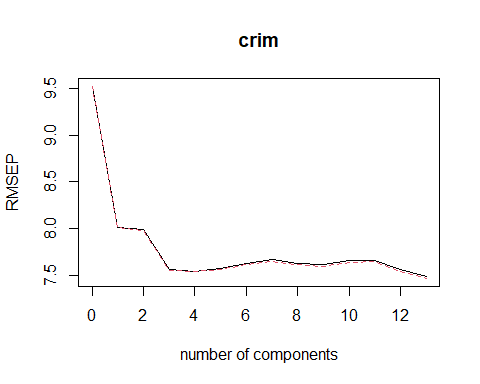
\includegraphics{STA_exam_ps33296_files/figure-latex/6.11.a-1.pdf}

\begin{Shaded}
\begin{Highlighting}[]
\NormalTok{pcr\_pred }\OtherTok{=} \FunctionTok{predict}\NormalTok{(pcr\_fit, dfTest, }\AttributeTok{ncomp=}\DecValTok{13}\NormalTok{)}

\NormalTok{MSE\_pcr }\OtherTok{=}\NormalTok{ (}\FunctionTok{mean}\NormalTok{((dfTest[, }\StringTok{"crim"}\NormalTok{] }\SpecialCharTok{{-}}\NormalTok{ pcr\_pred)}\SpecialCharTok{\^{}}\DecValTok{2}\NormalTok{))}
\FunctionTok{cat}\NormalTok{(MSE\_pcr)}
\end{Highlighting}
\end{Shaded}

\begin{verbatim}
## 18.4379
\end{verbatim}

\begin{Shaded}
\begin{Highlighting}[]
\FunctionTok{summary}\NormalTok{(pcr\_fit)}
\end{Highlighting}
\end{Shaded}

\begin{verbatim}
## Data:    X dimension: 354 13 
##  Y dimension: 354 1
## Fit method: svdpc
## Number of components considered: 13
## 
## VALIDATION: RMSEP
## Cross-validated using 10 random segments.
##        (Intercept)  1 comps  2 comps  3 comps  4 comps  5 comps  6 comps
## CV           9.525    8.011    7.987    7.559    7.543    7.573    7.627
## adjCV        9.525    8.008    7.984    7.554    7.537    7.566    7.617
##        7 comps  8 comps  9 comps  10 comps  11 comps  12 comps  13 comps
## CV       7.665    7.630    7.612     7.656     7.662     7.564     7.488
## adjCV    7.652    7.616    7.594     7.636     7.643     7.542     7.467
## 
## TRAINING: % variance explained
##       1 comps  2 comps  3 comps  4 comps  5 comps  6 comps  7 comps  8 comps
## X       48.58    61.36    70.50    77.35    83.36    88.23    91.30    93.45
## crim    29.82    30.41    37.81    38.42    38.54    38.72    39.17    40.09
##       9 comps  10 comps  11 comps  12 comps  13 comps
## X       95.54     97.16     98.50     99.54    100.00
## crim    41.44     41.62     41.62     43.09     44.25
\end{verbatim}

\begin{Shaded}
\begin{Highlighting}[]
\FunctionTok{barplot}\NormalTok{(}\FunctionTok{c}\NormalTok{(MSE\_stepwise\_lm, MSE\_ridge, MSE\_lasso, MSE\_pcr), }\AttributeTok{names.arg=}\FunctionTok{c}\NormalTok{(}\StringTok{"OLS"}\NormalTok{, }\StringTok{"Ridge"}\NormalTok{, }\StringTok{"Lasso"}\NormalTok{, }\StringTok{"PCR"}\NormalTok{), }\AttributeTok{main=}\StringTok{"MSE"}\NormalTok{)}
\end{Highlighting}
\end{Shaded}

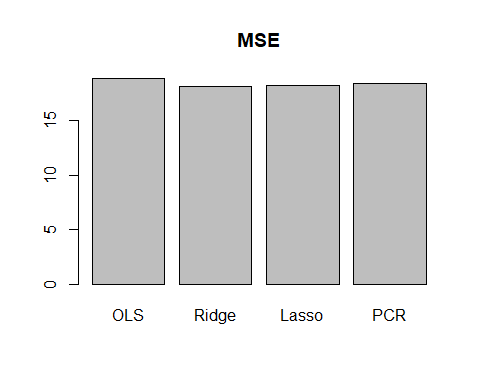
\includegraphics{STA_exam_ps33296_files/figure-latex/6.11.a-2.pdf}

Stepwise regression and lasso don't consider chas, tax, indus, zn and
black significant while predicting crime rate. Rad and Nox tend to be
the most significant predictors for crime rate. While Ridge gives the
best out of sample MSE. Lasso and Ridge show the lowest MSE.

\hypertarget{b-propose-a-model-or-set-of-models-that-seem-to-perform-well-on-this-data-set-and-justify-your-answer.-make-sure-that-you-are-evaluating-model-performance-using-validation-set-error-crossvalidation-or-some-other-reasonable-alternative-as-opposed-to-using-training-error.}{%
\paragraph{(b) Propose a model (or set of models) that seem to perform
well on this data set, and justify your answer. Make sure that you are
evaluating model performance using validation set error,
crossvalidation, or some other reasonable alternative, as opposed to
using training
error.}\label{b-propose-a-model-or-set-of-models-that-seem-to-perform-well-on-this-data-set-and-justify-your-answer.-make-sure-that-you-are-evaluating-model-performance-using-validation-set-error-crossvalidation-or-some-other-reasonable-alternative-as-opposed-to-using-training-error.}}

Based on the above models, we would choose Ridge/Lasso as the best model
as it gives the lowest MSE. The MSE is calculated on the test sample and
we have used cross validation to confirm that the model does not overfit
on the training data.

\hypertarget{c-does-your-chosen-model-involve-all-of-the-features-in-the-dataset-why-or-why-not}{%
\paragraph{(c) Does your chosen model involve all of the features in the
dataset? Why or why
not?}\label{c-does-your-chosen-model-involve-all-of-the-features-in-the-dataset-why-or-why-not}}

Our model doesnt use all variables, especially Lasso removed the `age'
predictor as it doesnt show any significant impact on crime rate. On
similar lines, tax, black, indx and zn also have a very low value (near
zero), so the impact of these variables can also be ignored.

\begin{center}\rule{0.5\linewidth}{0.5pt}\end{center}

\hypertarget{chapter-8}{%
\section{Chapter 8}\label{chapter-8}}

\hypertarget{question-8}{%
\subsubsection{Question 8}\label{question-8}}

We will seek to predict Sales using regression trees and related
approaches, treating the response as a quantitative variable.

\hypertarget{a-split-the-data-set-into-a-training-set-and-a-test-set.-1}{%
\paragraph{(a) Split the data set into a training set and a test
set.}\label{a-split-the-data-set-into-a-training-set-and-a-test-set.-1}}

\begin{Shaded}
\begin{Highlighting}[]
\FunctionTok{rm}\NormalTok{(}\AttributeTok{list =} \FunctionTok{ls}\NormalTok{())}
\FunctionTok{library}\NormalTok{(ISLR)}
\FunctionTok{library}\NormalTok{(tidyverse)}
\FunctionTok{library}\NormalTok{(rpart)}
\FunctionTok{library}\NormalTok{(tree)}
\FunctionTok{library}\NormalTok{(randomForest)}
\FunctionTok{set.seed}\NormalTok{(}\DecValTok{101}\NormalTok{)}

\NormalTok{carseats\_dat }\OtherTok{=}\NormalTok{ Carseats}

\CommentTok{\# splitting dataset with 70:30 split (train{-}test)}
\NormalTok{n }\OtherTok{=}\NormalTok{ carseats\_dat }\SpecialCharTok{\%\textgreater{}\%}\NormalTok{ nrow}
\NormalTok{idx }\OtherTok{=} \FunctionTok{sample}\NormalTok{(}\DecValTok{1}\SpecialCharTok{:}\NormalTok{n, }\FloatTok{0.7}\SpecialCharTok{*}\NormalTok{n)}


\NormalTok{train }\OtherTok{=}\NormalTok{ carseats\_dat[idx,]}
\CommentTok{\# length of training set}
\FunctionTok{nrow}\NormalTok{(train)}
\end{Highlighting}
\end{Shaded}

\begin{verbatim}
## [1] 280
\end{verbatim}

\begin{Shaded}
\begin{Highlighting}[]
\NormalTok{test }\OtherTok{=}\NormalTok{ carseats\_dat[}\SpecialCharTok{{-}}\NormalTok{idx,]}
\CommentTok{\# length of testing set}
\FunctionTok{nrow}\NormalTok{(test)}
\end{Highlighting}
\end{Shaded}

\begin{verbatim}
## [1] 120
\end{verbatim}

\hypertarget{b-fit-a-regression-tree-to-the-training-set.-plot-the-tree-and-interpret-the-results.-what-test-error-rate-do-you-obtain}{%
\paragraph{(b) Fit a regression tree to the training set. Plot the tree,
and interpret the results. What test error rate do you
obtain?}\label{b-fit-a-regression-tree-to-the-training-set.-plot-the-tree-and-interpret-the-results.-what-test-error-rate-do-you-obtain}}

\begin{Shaded}
\begin{Highlighting}[]
\NormalTok{train }\SpecialCharTok{\%\textgreater{}\%}\NormalTok{ str}
\end{Highlighting}
\end{Shaded}

\begin{verbatim}
## 'data.frame':    280 obs. of  11 variables:
##  $ Sales      : num  3.15 6.8 8.39 7.78 8.64 ...
##  $ CompPrice  : num  117 137 115 86 111 122 133 114 133 125 ...
##  $ Income     : num  66 117 97 54 101 36 33 43 31 48 ...
##  $ Advertising: num  1 5 5 0 17 5 10 0 1 3 ...
##  $ Population : num  65 337 134 497 266 369 333 199 80 192 ...
##  $ Price      : num  111 135 84 64 91 72 129 88 145 116 ...
##  $ ShelveLoc  : Factor w/ 3 levels "Bad","Good","Medium": 1 1 1 1 3 2 2 2 3 3 ...
##  $ Age        : num  55 38 55 33 63 35 71 57 42 51 ...
##  $ Education  : num  11 10 11 12 17 10 14 10 18 14 ...
##  $ Urban      : Factor w/ 2 levels "No","Yes": 2 2 2 2 1 2 2 1 2 2 ...
##  $ US         : Factor w/ 2 levels "No","Yes": 2 2 2 1 2 2 2 2 2 2 ...
\end{verbatim}

\begin{Shaded}
\begin{Highlighting}[]
\NormalTok{tree\_fit }\OtherTok{=} \FunctionTok{tree}\NormalTok{(Sales }\SpecialCharTok{\textasciitilde{}}\NormalTok{ ., }\AttributeTok{data =}\NormalTok{ train)}

\FunctionTok{summary}\NormalTok{(tree\_fit)}
\end{Highlighting}
\end{Shaded}

\begin{verbatim}
## 
## Regression tree:
## tree(formula = Sales ~ ., data = train)
## Variables actually used in tree construction:
## [1] "ShelveLoc"   "Price"       "Age"         "Income"      "Advertising"
## [6] "CompPrice"   "US"         
## Number of terminal nodes:  14 
## Residual mean deviance:  2.689 = 715.3 / 266 
## Distribution of residuals:
##    Min. 1st Qu.  Median    Mean 3rd Qu.    Max. 
##  -4.355  -1.041   0.006   0.000   1.000   4.905
\end{verbatim}

\begin{Shaded}
\begin{Highlighting}[]
\FunctionTok{plot}\NormalTok{(tree\_fit)}
\FunctionTok{text}\NormalTok{(tree\_fit, }\AttributeTok{pretty=}\DecValTok{0}\NormalTok{)}
\end{Highlighting}
\end{Shaded}

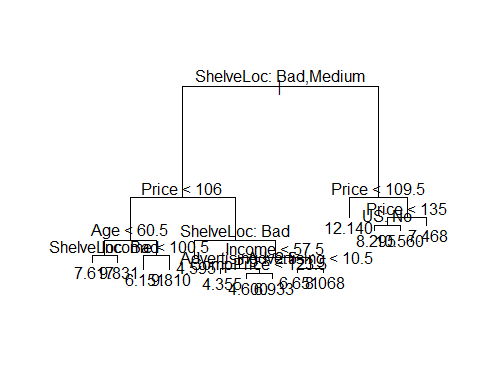
\includegraphics{STA_exam_ps33296_files/figure-latex/8.8.b-1.pdf}

\begin{Shaded}
\begin{Highlighting}[]
\NormalTok{pred\_tree }\OtherTok{=} \FunctionTok{predict}\NormalTok{(tree\_fit, test}\SpecialCharTok{\%\textgreater{}\%}\NormalTok{dplyr}\SpecialCharTok{::}\FunctionTok{select}\NormalTok{(}\SpecialCharTok{{-}}\NormalTok{Sales))}
\NormalTok{MSE\_tree }\OtherTok{=} \FunctionTok{mean}\NormalTok{((test[,}\StringTok{\textquotesingle{}Sales\textquotesingle{}}\NormalTok{] }\SpecialCharTok{{-}}\NormalTok{ pred\_tree)}\SpecialCharTok{\^{}}\DecValTok{2}\NormalTok{)}
\FunctionTok{cat}\NormalTok{(MSE\_tree)}
\end{Highlighting}
\end{Shaded}

\begin{verbatim}
## 4.915969
\end{verbatim}

\hypertarget{c-use-cross-validation-in-order-to-determine-the-optimal-level-of-tree-complexity.-does-pruning-the-tree-improve-the-test-error-rate}{%
\paragraph{(c) Use cross-validation in order to determine the optimal
level of tree complexity. Does pruning the tree improve the test error
rate?}\label{c-use-cross-validation-in-order-to-determine-the-optimal-level-of-tree-complexity.-does-pruning-the-tree-improve-the-test-error-rate}}

\begin{Shaded}
\begin{Highlighting}[]
\NormalTok{cv\_tree\_fit }\OtherTok{=} \FunctionTok{cv.tree}\NormalTok{(tree\_fit, }\AttributeTok{FUN =}\NormalTok{ prune.tree)}
\FunctionTok{par}\NormalTok{(}\AttributeTok{mfrow =} \FunctionTok{c}\NormalTok{(}\DecValTok{1}\NormalTok{, }\DecValTok{2}\NormalTok{))}
\FunctionTok{plot}\NormalTok{(cv\_tree\_fit}\SpecialCharTok{$}\NormalTok{size, cv\_tree\_fit}\SpecialCharTok{$}\NormalTok{dev, }\AttributeTok{type =} \StringTok{"b"}\NormalTok{)}
\FunctionTok{plot}\NormalTok{(cv\_tree\_fit}\SpecialCharTok{$}\NormalTok{k, cv\_tree\_fit}\SpecialCharTok{$}\NormalTok{dev, }\AttributeTok{type =} \StringTok{"b"}\NormalTok{)}
\end{Highlighting}
\end{Shaded}

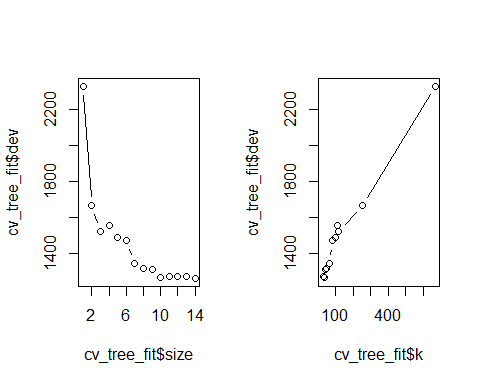
\includegraphics{STA_exam_ps33296_files/figure-latex/8.8.c-1.pdf}

\begin{Shaded}
\begin{Highlighting}[]
\NormalTok{pruned\_tree }\OtherTok{=} \FunctionTok{prune.tree}\NormalTok{(tree\_fit, }\AttributeTok{best =} \DecValTok{8}\NormalTok{)}
\FunctionTok{par}\NormalTok{(}\AttributeTok{mfrow =} \FunctionTok{c}\NormalTok{(}\DecValTok{1}\NormalTok{, }\DecValTok{1}\NormalTok{))}
\FunctionTok{plot}\NormalTok{(pruned\_tree)}
\FunctionTok{text}\NormalTok{(pruned\_tree, }\AttributeTok{pretty =} \DecValTok{0}\NormalTok{)}
\end{Highlighting}
\end{Shaded}

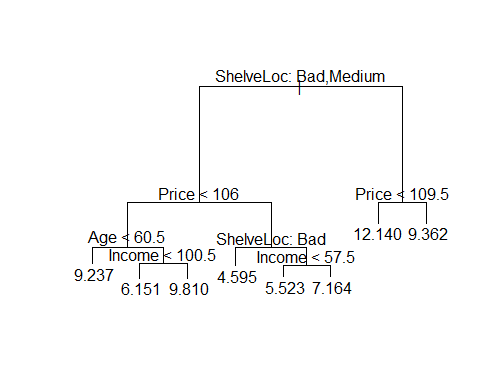
\includegraphics{STA_exam_ps33296_files/figure-latex/8.8.c-2.pdf}

\begin{Shaded}
\begin{Highlighting}[]
\NormalTok{pred\_pruned\_tree }\OtherTok{=} \FunctionTok{predict}\NormalTok{(pruned\_tree, test}\SpecialCharTok{\%\textgreater{}\%}\NormalTok{dplyr}\SpecialCharTok{::}\FunctionTok{select}\NormalTok{(}\SpecialCharTok{{-}}\NormalTok{Sales))}
\NormalTok{MSE\_pruned\_tree }\OtherTok{=} \FunctionTok{mean}\NormalTok{((test[,}\StringTok{\textquotesingle{}Sales\textquotesingle{}}\NormalTok{] }\SpecialCharTok{{-}}\NormalTok{ pred\_pruned\_tree)}\SpecialCharTok{\^{}}\DecValTok{2}\NormalTok{)}
\FunctionTok{cat}\NormalTok{(MSE\_pruned\_tree)}
\end{Highlighting}
\end{Shaded}

\begin{verbatim}
## 5.106689
\end{verbatim}

Pruning the tree increases test MSE.

\hypertarget{d-use-the-bagging-approach-in-order-to-analyze-this-data.-what-test-error-rate-do-you-obtain-use-the-importance-function-to-determine-which-variables-are-most-important}{%
\paragraph{(d) Use the bagging approach in order to analyze this data.
What test error rate do you obtain? Use the importance() function to
determine which variables are most
important}\label{d-use-the-bagging-approach-in-order-to-analyze-this-data.-what-test-error-rate-do-you-obtain-use-the-importance-function-to-determine-which-variables-are-most-important}}

\begin{Shaded}
\begin{Highlighting}[]
\NormalTok{rf\_fit }\OtherTok{=} \FunctionTok{randomForest}\NormalTok{(Sales }\SpecialCharTok{\textasciitilde{}}\NormalTok{ ., }\AttributeTok{data =}\NormalTok{ train, }\AttributeTok{importance =}\NormalTok{ T)}
\NormalTok{rf\_prediction }\OtherTok{=} \FunctionTok{predict}\NormalTok{(rf\_fit, test}\SpecialCharTok{\%\textgreater{}\%}\NormalTok{dplyr}\SpecialCharTok{::}\FunctionTok{select}\NormalTok{(}\SpecialCharTok{{-}}\NormalTok{Sales))}
\NormalTok{MSE\_rf }\OtherTok{=} \FunctionTok{mean}\NormalTok{((test[,}\StringTok{\textquotesingle{}Sales\textquotesingle{}}\NormalTok{] }\SpecialCharTok{{-}}\NormalTok{ rf\_prediction)}\SpecialCharTok{\^{}}\DecValTok{2}\NormalTok{)}
\FunctionTok{cat}\NormalTok{(MSE\_rf)}
\end{Highlighting}
\end{Shaded}

\begin{verbatim}
## 2.894636
\end{verbatim}

\begin{Shaded}
\begin{Highlighting}[]
\FunctionTok{importance}\NormalTok{(rf\_fit)}
\end{Highlighting}
\end{Shaded}

\begin{verbatim}
##                %IncMSE IncNodePurity
## CompPrice   12.0172360     188.31225
## Income       4.3452176     161.48257
## Advertising 16.2440037     189.68633
## Population  -1.8003869     145.20881
## Price       41.5614700     551.43929
## ShelveLoc   53.6475512     595.48634
## Age         14.5508718     212.65730
## Education    2.8477140      90.99886
## Urban        0.9014082      18.58106
## US           6.2667113      34.31104
\end{verbatim}

Random forest/bagging decreases the MSE and improves the model. Most
important variables are - ShelveLoc, Price and Advertising.

\hypertarget{e-use-random-forests-to-analyze-this-data.-what-test-error-rate-do-you-obtain-use-the-importance-function-to-determine-which-variables-are-most-important.-describe-the-effect-of-m-the-number-of-variables-considered-at-each-split-on-the-error-rate-obtained.}{%
\paragraph{(e) Use random forests to analyze this data. What test error
rate do you obtain? Use the importance() function to determine which
variables are most important. Describe the effect of m, the number of
variables considered at each split, on the error rate
obtained.}\label{e-use-random-forests-to-analyze-this-data.-what-test-error-rate-do-you-obtain-use-the-importance-function-to-determine-which-variables-are-most-important.-describe-the-effect-of-m-the-number-of-variables-considered-at-each-split-on-the-error-rate-obtained.}}

\begin{Shaded}
\begin{Highlighting}[]
\NormalTok{rf\_fit }\OtherTok{=} \FunctionTok{randomForest}\NormalTok{(Sales }\SpecialCharTok{\textasciitilde{}}\NormalTok{ ., }\AttributeTok{data =}\NormalTok{ train, }\AttributeTok{importance =}\NormalTok{ T, }\AttributeTok{mtry=}\DecValTok{3}\NormalTok{) }\CommentTok{\#increasing mtry improves the model}
\NormalTok{rf\_prediction }\OtherTok{=} \FunctionTok{predict}\NormalTok{(rf\_fit, test}\SpecialCharTok{\%\textgreater{}\%}\NormalTok{dplyr}\SpecialCharTok{::}\FunctionTok{select}\NormalTok{(}\SpecialCharTok{{-}}\NormalTok{Sales))}
\NormalTok{MSE\_rf }\OtherTok{=} \FunctionTok{mean}\NormalTok{((test[,}\StringTok{\textquotesingle{}Sales\textquotesingle{}}\NormalTok{] }\SpecialCharTok{{-}}\NormalTok{ rf\_prediction)}\SpecialCharTok{\^{}}\DecValTok{2}\NormalTok{)}
\FunctionTok{cat}\NormalTok{(MSE\_rf)}
\end{Highlighting}
\end{Shaded}

\begin{verbatim}
## 2.89402
\end{verbatim}

\begin{Shaded}
\begin{Highlighting}[]
\FunctionTok{importance}\NormalTok{(rf\_fit)}
\end{Highlighting}
\end{Shaded}

\begin{verbatim}
##                %IncMSE IncNodePurity
## CompPrice   12.3805867     188.26368
## Income       4.8364380     163.25233
## Advertising 16.8711925     189.02767
## Population   1.7622390     149.02625
## Price       44.5486037     555.36330
## ShelveLoc   51.4840070     593.38685
## Age         13.1179172     208.79060
## Education    1.5734843      84.82362
## Urban        0.3589163      19.50490
## US           4.9611884      32.36192
\end{verbatim}

Increasing mtry (sampling number of columns), improves the model and
decreases the MSE.

\begin{center}\rule{0.5\linewidth}{0.5pt}\end{center}

\hypertarget{chapter-8-1}{%
\section{Chapter 8}\label{chapter-8-1}}

\hypertarget{question-11-1}{%
\subsubsection{Question 11}\label{question-11-1}}

This question uses the Caravan data set.

\hypertarget{a-create-a-training-set-consisting-of-the-first-1000-observations-and-a-test-set-consisting-of-the-remaining-observations.}{%
\paragraph{(a) Create a training set consisting of the first 1,000
observations, and a test set consisting of the remaining
observations.}\label{a-create-a-training-set-consisting-of-the-first-1000-observations-and-a-test-set-consisting-of-the-remaining-observations.}}

\begin{Shaded}
\begin{Highlighting}[]
\FunctionTok{rm}\NormalTok{(}\AttributeTok{list =} \FunctionTok{ls}\NormalTok{())}
\FunctionTok{library}\NormalTok{(ISLR)}
\FunctionTok{library}\NormalTok{(tidyverse)}
\FunctionTok{library}\NormalTok{(gbm)}
\FunctionTok{set.seed}\NormalTok{(}\DecValTok{107}\NormalTok{)}

\NormalTok{caravan\_dat }\OtherTok{=}\NormalTok{ Caravan}
\CommentTok{\# caravan\_dat \%\textgreater{}\% str}
\NormalTok{caravan\_dat }\OtherTok{=}\NormalTok{ caravan\_dat }\SpecialCharTok{\%\textgreater{}\%} \FunctionTok{mutate}\NormalTok{(}\AttributeTok{purchase\_label =} \FunctionTok{ifelse}\NormalTok{(Purchase }\SpecialCharTok{==} \StringTok{"Yes"}\NormalTok{, }\DecValTok{1}\NormalTok{, }\DecValTok{0}\NormalTok{))}
\NormalTok{caravan\_dat }\OtherTok{=}\NormalTok{ caravan\_dat }\SpecialCharTok{\%\textgreater{}\%}\NormalTok{ dplyr}\SpecialCharTok{::}\FunctionTok{select}\NormalTok{(}\SpecialCharTok{{-}}\NormalTok{Purchase)}

\NormalTok{train }\OtherTok{=}\NormalTok{ caravan\_dat[}\DecValTok{1}\SpecialCharTok{:}\DecValTok{1000}\NormalTok{,]}
\NormalTok{test }\OtherTok{=}\NormalTok{ caravan\_dat[}\DecValTok{1000}\SpecialCharTok{:}\FunctionTok{nrow}\NormalTok{(caravan\_dat),]}
\end{Highlighting}
\end{Shaded}

\hypertarget{b-fit-a-boosting-model-to-the-training-set-with-purchase-as-the-response-and-the-other-variables-as-predictors.-use-1000-trees-and-a-shrinkage-value-of-0.01.-which-predictors-appear-to-be-the-most-important}{%
\paragraph{(b) Fit a boosting model to the training set with Purchase as
the response and the other variables as predictors. Use 1,000 trees, and
a shrinkage value of 0.01. Which predictors appear to be the most
important?}\label{b-fit-a-boosting-model-to-the-training-set-with-purchase-as-the-response-and-the-other-variables-as-predictors.-use-1000-trees-and-a-shrinkage-value-of-0.01.-which-predictors-appear-to-be-the-most-important}}

\begin{Shaded}
\begin{Highlighting}[]
\NormalTok{gbm\_fit }\OtherTok{=} \FunctionTok{gbm}\NormalTok{(purchase\_label }\SpecialCharTok{\textasciitilde{}}\NormalTok{ ., }\AttributeTok{data =}\NormalTok{ train, }\AttributeTok{n.trees =} \DecValTok{1000}\NormalTok{, }\AttributeTok{shrinkage =} \FloatTok{0.01}\NormalTok{)}
\end{Highlighting}
\end{Shaded}

\begin{verbatim}
## Distribution not specified, assuming bernoulli ...
\end{verbatim}

\begin{Shaded}
\begin{Highlighting}[]
\FunctionTok{summary}\NormalTok{(gbm\_fit)}
\end{Highlighting}
\end{Shaded}

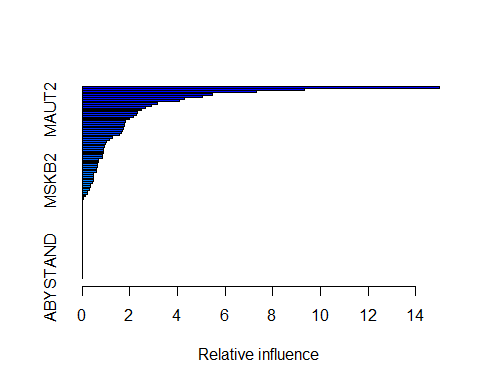
\includegraphics{STA_exam_ps33296_files/figure-latex/8.11.b-1.pdf}

\begin{verbatim}
##               var     rel.inf
## PPERSAUT PPERSAUT 15.00949288
## MKOOPKLA MKOOPKLA  9.31330624
## MOPLHOOG MOPLHOOG  7.31354135
## MBERMIDD MBERMIDD  5.46412685
## PBRAND     PBRAND  5.05350016
## MGODGE     MGODGE  4.27763318
## ABRAND     ABRAND  4.09160716
## MINK3045 MINK3045  3.16548232
## MOSTYPE   MOSTYPE  2.91321676
## MAUT1       MAUT1  2.63422368
## MAUT2       MAUT2  2.48588446
## MGODPR     MGODPR  2.33502437
## PWAPART   PWAPART  2.28073775
## MSKC         MSKC  2.14800637
## MBERHOOG MBERHOOG  1.97803947
## MSKA         MSKA  1.81351548
## PBYSTAND PBYSTAND  1.78416557
## MBERARBG MBERARBG  1.78266984
## MINKGEM   MINKGEM  1.74515538
## MRELGE     MRELGE  1.69242010
## MGODOV     MGODOV  1.62838163
## MSKB1       MSKB1  1.58201222
## MINK7512 MINK7512  1.26163756
## MRELOV     MRELOV  1.14516310
## MFGEKIND MFGEKIND  1.03379422
## MFWEKIND MFWEKIND  0.95475561
## MSKD         MSKD  0.93592796
## MBERBOER MBERBOER  0.89708790
## MHHUUR     MHHUUR  0.89375115
## MAUT0       MAUT0  0.87075206
## MGODRK     MGODRK  0.84551666
## MHKOOP     MHKOOP  0.83054456
## MZPART     MZPART  0.69206757
## MINKM30   MINKM30  0.67323829
## PMOTSCO   PMOTSCO  0.64292304
## MOSHOOFD MOSHOOFD  0.61773355
## MGEMLEEF MGEMLEEF  0.61396826
## MOPLMIDD MOPLMIDD  0.60766060
## MGEMOMV   MGEMOMV  0.48794508
## MINK4575 MINK4575  0.48236479
## PLEVEN     PLEVEN  0.46108039
## MSKB2       MSKB2  0.45895331
## APERSAUT APERSAUT  0.41358251
## MBERARBO MBERARBO  0.36397292
## MINK123M MINK123M  0.35758914
## MFALLEEN MFALLEEN  0.31913934
## MZFONDS   MZFONDS  0.22520830
## MRELSA     MRELSA  0.21865486
## MBERZELF MBERZELF  0.13429923
## MOPLLAAG MOPLLAAG  0.06854482
## MAANTHUI MAANTHUI  0.00000000
## PWABEDR   PWABEDR  0.00000000
## PWALAND   PWALAND  0.00000000
## PBESAUT   PBESAUT  0.00000000
## PVRAAUT   PVRAAUT  0.00000000
## PAANHANG PAANHANG  0.00000000
## PTRACTOR PTRACTOR  0.00000000
## PWERKT     PWERKT  0.00000000
## PBROM       PBROM  0.00000000
## PPERSONG PPERSONG  0.00000000
## PGEZONG   PGEZONG  0.00000000
## PWAOREG   PWAOREG  0.00000000
## PZEILPL   PZEILPL  0.00000000
## PPLEZIER PPLEZIER  0.00000000
## PFIETS     PFIETS  0.00000000
## PINBOED   PINBOED  0.00000000
## AWAPART   AWAPART  0.00000000
## AWABEDR   AWABEDR  0.00000000
## AWALAND   AWALAND  0.00000000
## ABESAUT   ABESAUT  0.00000000
## AMOTSCO   AMOTSCO  0.00000000
## AVRAAUT   AVRAAUT  0.00000000
## AAANHANG AAANHANG  0.00000000
## ATRACTOR ATRACTOR  0.00000000
## AWERKT     AWERKT  0.00000000
## ABROM       ABROM  0.00000000
## ALEVEN     ALEVEN  0.00000000
## APERSONG APERSONG  0.00000000
## AGEZONG   AGEZONG  0.00000000
## AWAOREG   AWAOREG  0.00000000
## AZEILPL   AZEILPL  0.00000000
## APLEZIER APLEZIER  0.00000000
## AFIETS     AFIETS  0.00000000
## AINBOED   AINBOED  0.00000000
## ABYSTAND ABYSTAND  0.00000000
\end{verbatim}

\textbf{PPERSAUT} and \textbf{MKOOPKLA} is the most important variables

\hypertarget{c-use-the-boosting-model-to-predict-the-response-on-the-test-data.-predict-that-a-person-will-make-a-purchase-if-the-estimated-probability-of-purchase-is-greater-than-20-.-form-a-confusion-matrix.-what-fraction-of-the-people-predicted-to-make-a-purchase-do-in-fact-make-one-how-does-this-compare-with-the-results-obtained-from-applying-knn-or-logistic-regression-to-this-data-set}{%
\paragraph{(c) Use the boosting model to predict the response on the
test data. Predict that a person will make a purchase if the estimated
probability of purchase is greater than 20 \%. Form a confusion matrix.
What fraction of the people predicted to make a purchase do in fact make
one? How does this compare with the results obtained from applying KNN
or logistic regression to this data
set?}\label{c-use-the-boosting-model-to-predict-the-response-on-the-test-data.-predict-that-a-person-will-make-a-purchase-if-the-estimated-probability-of-purchase-is-greater-than-20-.-form-a-confusion-matrix.-what-fraction-of-the-people-predicted-to-make-a-purchase-do-in-fact-make-one-how-does-this-compare-with-the-results-obtained-from-applying-knn-or-logistic-regression-to-this-data-set}}

\begin{Shaded}
\begin{Highlighting}[]
\FunctionTok{set.seed}\NormalTok{(}\DecValTok{123}\NormalTok{)}
\NormalTok{gbm\_prob }\OtherTok{=} \FunctionTok{predict}\NormalTok{(gbm\_fit, test }\SpecialCharTok{\%\textgreater{}\%}\NormalTok{ dplyr}\SpecialCharTok{::}\FunctionTok{select}\NormalTok{(}\SpecialCharTok{{-}}\NormalTok{purchase\_label), }\AttributeTok{type =}\StringTok{"response"}\NormalTok{)}
\NormalTok{gbm\_preds }\OtherTok{=} \FunctionTok{ifelse}\NormalTok{(gbm\_prob }\SpecialCharTok{\textgreater{}} \FloatTok{0.2}\NormalTok{, }\DecValTok{1}\NormalTok{, }\DecValTok{0}\NormalTok{)}
\FunctionTok{table}\NormalTok{(test}\SpecialCharTok{$}\NormalTok{purchase\_label, gbm\_preds)}
\end{Highlighting}
\end{Shaded}

\begin{verbatim}
##    gbm_preds
##        0    1
##   0 4425  109
##   1  257   32
\end{verbatim}

\begin{Shaded}
\begin{Highlighting}[]
\DecValTok{32}\SpecialCharTok{/}\NormalTok{(}\DecValTok{109} \SpecialCharTok{+} \DecValTok{32}\NormalTok{)}
\end{Highlighting}
\end{Shaded}

\begin{verbatim}
## [1] 0.2269504
\end{verbatim}

\begin{Shaded}
\begin{Highlighting}[]
\CommentTok{\# lm fit}
\NormalTok{lm\_fit }\OtherTok{=} \FunctionTok{lm}\NormalTok{(purchase\_label }\SpecialCharTok{\textasciitilde{}}\NormalTok{ ., }\AttributeTok{data =}\NormalTok{ train, }\AttributeTok{family =}\NormalTok{ binomial)}

\NormalTok{lm\_prob }\OtherTok{=} \FunctionTok{predict}\NormalTok{(lm\_fit, test }\SpecialCharTok{\%\textgreater{}\%}\NormalTok{ dplyr}\SpecialCharTok{::}\FunctionTok{select}\NormalTok{(}\SpecialCharTok{{-}}\NormalTok{purchase\_label), }\AttributeTok{type =}\StringTok{"response"}\NormalTok{)}
\NormalTok{lm\_preds }\OtherTok{=} \FunctionTok{ifelse}\NormalTok{(lm\_prob }\SpecialCharTok{\textgreater{}} \FloatTok{0.2}\NormalTok{, }\DecValTok{1}\NormalTok{, }\DecValTok{0}\NormalTok{)}
\FunctionTok{table}\NormalTok{(test}\SpecialCharTok{$}\NormalTok{purchase\_label, lm\_preds)}
\end{Highlighting}
\end{Shaded}

\begin{verbatim}
##    lm_preds
##        0    1
##   0 4407  127
##   1  253   36
\end{verbatim}

\begin{Shaded}
\begin{Highlighting}[]
\DecValTok{36}\SpecialCharTok{/}\NormalTok{(}\DecValTok{127}\SpecialCharTok{+}\DecValTok{36}\NormalTok{)}
\end{Highlighting}
\end{Shaded}

\begin{verbatim}
## [1] 0.2208589
\end{verbatim}

22.7\% are predicted to purchase in boosting compared to 22\% in glm
which is lower

\begin{center}\rule{0.5\linewidth}{0.5pt}\end{center}

\hypertarget{chapter-10}{%
\section{Chapter 10}\label{chapter-10}}

\hypertarget{question-7}{%
\subsubsection{Question 7}\label{question-7}}

In the chapter, we mentioned the use of correlation-based distance and
Euclidean distance as dissimilarity measures for hierarchical
clustering. It turns out that these two measures are almost equivalent:
if each observation has been centered to have mean zero and standard
deviation one, and if we let rij denote the correlation between the ith
and jth observations, then the quantity 1 − rij is proportional to the
squared Euclidean distance between the ith and jth observations. On the
USArrests data, show that this proportionality holds. Hint: The
Euclidean distance can be calculated using the dist() function, and
correlations can be calculated using the cor() function.

\begin{Shaded}
\begin{Highlighting}[]
\FunctionTok{rm}\NormalTok{(}\AttributeTok{list =} \FunctionTok{ls}\NormalTok{())}
\FunctionTok{library}\NormalTok{(ISLR)}
\FunctionTok{library}\NormalTok{(tidyverse)}

\FunctionTok{set.seed}\NormalTok{(}\DecValTok{108}\NormalTok{)}

\NormalTok{usarrests\_dat }\OtherTok{=}\NormalTok{ USArrests}
\NormalTok{usarrests\_dat }\SpecialCharTok{\%\textgreater{}\%}\NormalTok{ str}
\end{Highlighting}
\end{Shaded}

\begin{verbatim}
## 'data.frame':    50 obs. of  4 variables:
##  $ Murder  : num  13.2 10 8.1 8.8 9 7.9 3.3 5.9 15.4 17.4 ...
##  $ Assault : int  236 263 294 190 276 204 110 238 335 211 ...
##  $ UrbanPop: int  58 48 80 50 91 78 77 72 80 60 ...
##  $ Rape    : num  21.2 44.5 31 19.5 40.6 38.7 11.1 15.8 31.9 25.8 ...
\end{verbatim}

\begin{Shaded}
\begin{Highlighting}[]
\NormalTok{scaled\_US\_arrests }\OtherTok{=} \FunctionTok{scale}\NormalTok{(USArrests)}

\NormalTok{dist\_mat }\OtherTok{=} \FunctionTok{dist}\NormalTok{(}\FunctionTok{t}\NormalTok{(scaled\_US\_arrests))}

\CommentTok{\# These match with one another so they are in proportion}
\DecValTok{1} \SpecialCharTok{{-}} \FunctionTok{cor}\NormalTok{(usarrests\_dat)}
\end{Highlighting}
\end{Shaded}

\begin{verbatim}
##             Murder   Assault  UrbanPop      Rape
## Murder   0.0000000 0.1981267 0.9304274 0.4364212
## Assault  0.1981267 0.0000000 0.7411283 0.3347588
## UrbanPop 0.9304274 0.7411283 0.0000000 0.5886588
## Rape     0.4364212 0.3347588 0.5886588 0.0000000
\end{verbatim}

\begin{Shaded}
\begin{Highlighting}[]
\NormalTok{dist\_mat}\SpecialCharTok{\^{}}\DecValTok{2}
\end{Highlighting}
\end{Shaded}

\begin{verbatim}
##            Murder  Assault UrbanPop
## Assault  19.41642                  
## UrbanPop 91.18188 72.63057         
## Rape     42.76927 32.80636 57.68856
\end{verbatim}

\begin{center}\rule{0.5\linewidth}{0.5pt}\end{center}

\hypertarget{exam-problems}{%
\section{Exam Problems}\label{exam-problems}}

\hypertarget{problem-1-beauty-pays}{%
\subsubsection{Problem 1: Beauty Pays!}\label{problem-1-beauty-pays}}

\hypertarget{using-the-data-estimate-the-effect-of-beauty-into-course-ratings.-make-sure-to-think-about-the-potential-many-other-determinants.-describe-your-analysis-and-your-conclusions.}{%
\paragraph{1. Using the data, estimate the effect of ``beauty'' into
course ratings. Make sure to think about the potential many ``other
determinants''. Describe your analysis and your
conclusions.}\label{using-the-data-estimate-the-effect-of-beauty-into-course-ratings.-make-sure-to-think-about-the-potential-many-other-determinants.-describe-your-analysis-and-your-conclusions.}}

\begin{Shaded}
\begin{Highlighting}[]
\FunctionTok{rm}\NormalTok{(}\AttributeTok{list =} \FunctionTok{ls}\NormalTok{())}
\FunctionTok{library}\NormalTok{(tidyverse)}

\FunctionTok{set.seed}\NormalTok{(}\DecValTok{108}\NormalTok{)}

\NormalTok{beauty\_dat }\OtherTok{=} \FunctionTok{as.tibble}\NormalTok{(}\FunctionTok{read.csv}\NormalTok{(}\StringTok{"BeautyData.csv"}\NormalTok{))}

\NormalTok{lm\_fit }\OtherTok{=} \FunctionTok{lm}\NormalTok{(CourseEvals  }\SpecialCharTok{\textasciitilde{}}\NormalTok{., }\AttributeTok{data=}\NormalTok{beauty\_dat)}

\FunctionTok{summary}\NormalTok{(lm\_fit)}
\end{Highlighting}
\end{Shaded}

\begin{verbatim}
## 
## Call:
## lm(formula = CourseEvals ~ ., data = beauty_dat)
## 
## Residuals:
##      Min       1Q   Median       3Q      Max 
## -1.31385 -0.30202  0.01011  0.29815  1.04929 
## 
## Coefficients:
##             Estimate Std. Error t value Pr(>|t|)    
## (Intercept)  4.06542    0.05145  79.020  < 2e-16 ***
## BeautyScore  0.30415    0.02543  11.959  < 2e-16 ***
## female      -0.33199    0.04075  -8.146 3.62e-15 ***
## lower       -0.34255    0.04282  -7.999 1.04e-14 ***
## nonenglish  -0.25808    0.08478  -3.044  0.00247 ** 
## tenuretrack -0.09945    0.04888  -2.035  0.04245 *  
## ---
## Signif. codes:  0 '***' 0.001 '**' 0.01 '*' 0.05 '.' 0.1 ' ' 1
## 
## Residual standard error: 0.4273 on 457 degrees of freedom
## Multiple R-squared:  0.3471, Adjusted R-squared:  0.3399 
## F-statistic: 48.58 on 5 and 457 DF,  p-value: < 2.2e-16
\end{verbatim}

\begin{itemize}
\tightlist
\item
  BeautyScore, female, lower and nonenglish are all significant while
  predicting the Evaluation Score
\item
  Beauty affects the evaluation scores significantly
\item
  Females score lower in evaluations - there is no possible explanation
  for this
\item
  non-english speakers will have difficult time in communicating ideas
  so the scores for them will be lower
\item
  evaluations from lower division classes are less, because people
  taking these classes might not be interested in them
\end{itemize}

\hypertarget{in-his-paper-dr.-hamermesh-has-the-following-sentence-disentangling-whether-this-outcome-represents-productivity-or-discrimination-is-as-with-the-issue-generally-probably-impossible.-using-the-concepts-we-have-talked-about-so-far-what-does-he-mean-by-that}{%
\paragraph{2. In his paper, Dr.~Hamermesh has the following sentence:
``Disentangling whether this outcome represents productivity or
discrimination is, as with the issue generally, probably impossible''.
Using the concepts we have talked about so far, what does he mean by
that?}\label{in-his-paper-dr.-hamermesh-has-the-following-sentence-disentangling-whether-this-outcome-represents-productivity-or-discrimination-is-as-with-the-issue-generally-probably-impossible.-using-the-concepts-we-have-talked-about-so-far-what-does-he-mean-by-that}}

One cannot say with certainty that Beauty affects evaluation scores,
there appears to be discrimination against females. But all in all there
are many other factors that influence evaluation scores like english
speaking, teaching lower division subjects etc. which can affect beauty
according to the summary of regression model fit shown in the previous
answer

\begin{center}\rule{0.5\linewidth}{0.5pt}\end{center}

\hypertarget{problem-2-housing-price-structure}{%
\subsubsection{Problem 2: Housing Price
Structure}\label{problem-2-housing-price-structure}}

The file MidCity.xls, available on the class website, contains data on
128 recent sales of houses in a town. For each sale, the file shows the
neighborhood in which the house is located, the number of offers made on
the house, the square footage, whether the house is made out of brick,
the number of bathrooms, the number of bedrooms, and the selling price.
Neighborhoods 1 and 2 are more traditional whereas 3 is a more modern,
newer and more prestigious part of town. Use regression models to
estimate the pricing structure of houses in this town and answer the
following questions

\hypertarget{is-there-a-premium-for-brick-houses-everything-else-being-equal}{%
\paragraph{1. Is there a premium for brick houses everything else being
equal?}\label{is-there-a-premium-for-brick-houses-everything-else-being-equal}}

\begin{Shaded}
\begin{Highlighting}[]
\FunctionTok{rm}\NormalTok{(}\AttributeTok{list =} \FunctionTok{ls}\NormalTok{())}
\FunctionTok{library}\NormalTok{(tidyverse)}
\FunctionTok{set.seed}\NormalTok{(}\DecValTok{111}\NormalTok{)}

\NormalTok{midcity\_dat }\OtherTok{=} \FunctionTok{as.tibble}\NormalTok{(}\FunctionTok{read.csv}\NormalTok{(}\StringTok{"MidCity.csv"}\NormalTok{))}
\CommentTok{\# midcity\_dat \%\textgreater{}\% str}

\NormalTok{midcity\_dat }\OtherTok{=}\NormalTok{ midcity\_dat }\SpecialCharTok{\%\textgreater{}\%} \FunctionTok{mutate}\NormalTok{(}\AttributeTok{Brick =} \FunctionTok{ifelse}\NormalTok{(Brick }\SpecialCharTok{==} \StringTok{"Yes"}\NormalTok{,}\DecValTok{1}\NormalTok{,}\DecValTok{0}\NormalTok{))}

\NormalTok{midcity\_dat}
\end{Highlighting}
\end{Shaded}

\begin{verbatim}
## # A tibble: 128 x 8
##     Home  Nbhd Offers  SqFt Brick Bedrooms Bathrooms  Price
##    <int> <int>  <int> <int> <dbl>    <int>     <int>  <int>
##  1     1     2      2  1790     0        2         2 114300
##  2     2     2      3  2030     0        4         2 114200
##  3     3     2      1  1740     0        3         2 114800
##  4     4     2      3  1980     0        3         2  94700
##  5     5     2      3  2130     0        3         3 119800
##  6     6     1      2  1780     0        3         2 114600
##  7     7     3      3  1830     1        3         3 151600
##  8     8     3      2  2160     0        4         2 150700
##  9     9     2      3  2110     0        4         2 119200
## 10    10     2      3  1730     0        3         3 104000
## # ... with 118 more rows
\end{verbatim}

\begin{Shaded}
\begin{Highlighting}[]
\NormalTok{lm\_fit }\OtherTok{=} \FunctionTok{lm}\NormalTok{(Price  }\SpecialCharTok{\textasciitilde{}}\NormalTok{ ., }\AttributeTok{data=}\NormalTok{midcity\_dat)}

\FunctionTok{summary}\NormalTok{(lm\_fit)}
\end{Highlighting}
\end{Shaded}

\begin{verbatim}
## 
## Call:
## lm(formula = Price ~ ., data = midcity_dat)
## 
## Residuals:
##      Min       1Q   Median       3Q      Max 
## -24940.6  -8383.0    430.7   7430.4  31371.2 
## 
## Coefficients:
##              Estimate Std. Error t value Pr(>|t|)    
## (Intercept) -9814.663   9858.884  -0.996  0.32149    
## Home            6.187     28.973   0.214  0.83128    
## Nbhd         9832.281   1821.869   5.397 3.47e-07 ***
## Offers      -8351.794   1267.428  -6.590 1.24e-09 ***
## SqFt           49.811      6.769   7.359 2.53e-11 ***
## Brick       15601.818   2261.896   6.898 2.66e-10 ***
## Bedrooms     5671.911   1840.979   3.081  0.00256 ** 
## Bathrooms    8243.545   2449.897   3.365  0.00103 ** 
## ---
## Signif. codes:  0 '***' 0.001 '**' 0.01 '*' 0.05 '.' 0.1 ' ' 1
## 
## Residual standard error: 11540 on 120 degrees of freedom
## Multiple R-squared:  0.8256, Adjusted R-squared:  0.8154 
## F-statistic: 81.15 on 7 and 120 DF,  p-value: < 2.2e-16
\end{verbatim}

People are willing to play premium for a brick home. As Brick is +ve in
the summary of lm\_fit and its p-value \textless{} 0.05 which makes it
significant.

\hypertarget{is-there-a-premium-for-houses-in-neighborhood-3}{%
\paragraph{2. Is there a premium for houses in neighborhood
3?}\label{is-there-a-premium-for-houses-in-neighborhood-3}}

\begin{Shaded}
\begin{Highlighting}[]
\CommentTok{\# adding dummy for neighborhood 3}
\NormalTok{midcity\_dat }\OtherTok{=}\NormalTok{ midcity\_dat }\SpecialCharTok{\%\textgreater{}\%} \FunctionTok{mutate}\NormalTok{(}\AttributeTok{Nbhd3 =} \FunctionTok{ifelse}\NormalTok{(Nbhd }\SpecialCharTok{==} \DecValTok{3}\NormalTok{,}\DecValTok{1}\NormalTok{,}\DecValTok{0}\NormalTok{))}

\NormalTok{lm\_fit }\OtherTok{=} \FunctionTok{lm}\NormalTok{(Price  }\SpecialCharTok{\textasciitilde{}}\NormalTok{ ., }\AttributeTok{data=}\NormalTok{midcity\_dat)}

\FunctionTok{summary}\NormalTok{(lm\_fit)}
\end{Highlighting}
\end{Shaded}

\begin{verbatim}
## 
## Call:
## lm(formula = Price ~ ., data = midcity_dat)
## 
## Residuals:
##      Min       1Q   Median       3Q      Max 
## -27897.8  -6074.8    -48.7   5551.8  27536.4 
## 
## Coefficients:
##              Estimate Std. Error t value Pr(>|t|)    
## (Intercept)  3767.339   8854.757   0.425 0.671270    
## Home          -11.456     25.387  -0.451 0.652616    
## Nbhd        -1729.613   2433.756  -0.711 0.478675    
## Offers      -8350.128   1103.693  -7.566 8.96e-12 ***
## SqFt           53.634      5.926   9.051 3.30e-15 ***
## Brick       17313.540   1988.548   8.707 2.12e-14 ***
## Bedrooms     4136.461   1621.775   2.551 0.012023 *  
## Bathrooms    7975.157   2133.831   3.737 0.000287 ***
## Nbhd3       23993.932   3830.057   6.265 6.17e-09 ***
## ---
## Signif. codes:  0 '***' 0.001 '**' 0.01 '*' 0.05 '.' 0.1 ' ' 1
## 
## Residual standard error: 10050 on 119 degrees of freedom
## Multiple R-squared:  0.8688, Adjusted R-squared:   0.86 
## F-statistic: 98.54 on 8 and 119 DF,  p-value: < 2.2e-16
\end{verbatim}

There is a premium for Neighborhood 3. Dummy variable Nbhd3 is positive
and has a p-value \textless{} 0.05 so it is statistically significant.

\hypertarget{is-there-an-extra-premium-for-brick-houses-in-neighborhood-3}{%
\paragraph{3. Is there an extra premium for brick houses in neighborhood
3?}\label{is-there-an-extra-premium-for-brick-houses-in-neighborhood-3}}

\begin{Shaded}
\begin{Highlighting}[]
\CommentTok{\# adding dummy for neighborhood 3 and brick houses}
\NormalTok{midcity\_dat }\OtherTok{=}\NormalTok{ midcity\_dat }\SpecialCharTok{\%\textgreater{}\%} \FunctionTok{mutate}\NormalTok{(}\AttributeTok{Nbhd3\_brick =} \FunctionTok{ifelse}\NormalTok{((Nbhd }\SpecialCharTok{==} \DecValTok{3}\NormalTok{) }\SpecialCharTok{\&}\NormalTok{ (Brick }\SpecialCharTok{==} \DecValTok{1}\NormalTok{),}\DecValTok{1}\NormalTok{, }\DecValTok{0}\NormalTok{))}


\NormalTok{lm\_fit }\OtherTok{=} \FunctionTok{lm}\NormalTok{(Price  }\SpecialCharTok{\textasciitilde{}}\NormalTok{ ., }\AttributeTok{data=}\NormalTok{midcity\_dat)}

\FunctionTok{summary}\NormalTok{(lm\_fit)}
\end{Highlighting}
\end{Shaded}

\begin{verbatim}
## 
## Call:
## lm(formula = Price ~ ., data = midcity_dat)
## 
## Residuals:
##      Min       1Q   Median       3Q      Max 
## -27515.9  -5681.0   -459.6   4451.0  26695.6 
## 
## Coefficients:
##              Estimate Std. Error t value Pr(>|t|)    
## (Intercept)  3731.658   8676.193   0.430  0.66791    
## Home          -11.799     24.875  -0.474  0.63613    
## Nbhd         -846.146   2412.025  -0.351  0.72636    
## Offers      -8486.348   1082.875  -7.837 2.26e-12 ***
## SqFt           54.726      5.823   9.397 5.36e-16 ***
## Brick       13839.320   2413.580   5.734 7.69e-08 ***
## Bedrooms     4605.046   1600.639   2.877  0.00477 ** 
## Bathrooms    6556.432   2170.200   3.021  0.00309 ** 
## Nbhd3       18779.206   4319.105   4.348 2.93e-05 ***
## Nbhd3_brick 10192.783   4178.971   2.439  0.01621 *  
## ---
## Signif. codes:  0 '***' 0.001 '**' 0.01 '*' 0.05 '.' 0.1 ' ' 1
## 
## Residual standard error: 9850 on 118 degrees of freedom
## Multiple R-squared:  0.8751, Adjusted R-squared:  0.8656 
## F-statistic:  91.9 on 9 and 118 DF,  p-value: < 2.2e-16
\end{verbatim}

Nbhd3\_brick shows a statistical significance with 95\% confidence. So
neighborhood 3 with Brick houses do have a premium. But if we consider a
narrow confidence interval then it is not statistically significant.

\hypertarget{for-the-purposes-of-prediction-could-you-combine-the-neighborhoods-1-and-2-into-a-single-older-neighborhood}{%
\paragraph{4. For the purposes of prediction could you combine the
neighborhoods 1 and 2 into a single ``older''
neighborhood?}\label{for-the-purposes-of-prediction-could-you-combine-the-neighborhoods-1-and-2-into-a-single-older-neighborhood}}

\begin{Shaded}
\begin{Highlighting}[]
\CommentTok{\# adding dummy for neighborhood 3 and brick houses}
\NormalTok{midcity\_dat\_nbhd }\OtherTok{=}\NormalTok{ midcity\_dat }\SpecialCharTok{\%\textgreater{}\%} \FunctionTok{mutate}\NormalTok{(}\AttributeTok{Nbhd2 =} \FunctionTok{ifelse}\NormalTok{(Nbhd }\SpecialCharTok{==} \DecValTok{2}\NormalTok{, }\DecValTok{1}\NormalTok{, }\DecValTok{0}\NormalTok{), }\AttributeTok{Nbhd1 =} \FunctionTok{ifelse}\NormalTok{(Nbhd }\SpecialCharTok{==} \DecValTok{1}\NormalTok{, }\DecValTok{1}\NormalTok{, }\DecValTok{0}\NormalTok{)) }\SpecialCharTok{\%\textgreater{}\%}\NormalTok{ dplyr}\SpecialCharTok{::}\FunctionTok{select}\NormalTok{(}\SpecialCharTok{{-}}\FunctionTok{c}\NormalTok{(Nbhd3\_brick, Nbhd3, Nbhd, Nbhd1))}


\NormalTok{lm\_fit }\OtherTok{=} \FunctionTok{lm}\NormalTok{(Price  }\SpecialCharTok{\textasciitilde{}}\NormalTok{ ., }\AttributeTok{data=}\NormalTok{midcity\_dat\_nbhd)}

\FunctionTok{summary}\NormalTok{(lm\_fit)}
\end{Highlighting}
\end{Shaded}

\begin{verbatim}
## 
## Call:
## lm(formula = Price ~ ., data = midcity_dat_nbhd)
## 
## Residuals:
##    Min     1Q Median     3Q    Max 
## -32878  -6912   -437   7815  28888 
## 
## Coefficients:
##               Estimate Std. Error t value Pr(>|t|)    
## (Intercept) -14586.482   9877.166  -1.477 0.142352    
## Home           -28.215     29.234  -0.965 0.336426    
## Offers      -12380.356   1054.349 -11.742  < 2e-16 ***
## SqFt            63.781      6.615   9.642  < 2e-16 ***
## Brick        18837.295   2285.705   8.241 2.45e-13 ***
## Bedrooms      8341.788   1719.755   4.851 3.73e-06 ***
## Bathrooms     9714.695   2450.393   3.965 0.000125 ***
## Nbhd2       -11455.485   2214.702  -5.172 9.37e-07 ***
## ---
## Signif. codes:  0 '***' 0.001 '**' 0.01 '*' 0.05 '.' 0.1 ' ' 1
## 
## Residual standard error: 11640 on 120 degrees of freedom
## Multiple R-squared:  0.8228, Adjusted R-squared:  0.8124 
## F-statistic: 79.59 on 7 and 120 DF,  p-value: < 2.2e-16
\end{verbatim}

\begin{Shaded}
\begin{Highlighting}[]
\DecValTok{1650}\SpecialCharTok{/}\DecValTok{120}
\end{Highlighting}
\end{Shaded}

\begin{verbatim}
## [1] 13.75
\end{verbatim}

Nbhd2 is statistically significant and we cannot club it along with 1 as
`older'

\begin{center}\rule{0.5\linewidth}{0.5pt}\end{center}

\hypertarget{problem-3-what-causes-what}{%
\subsubsection{Problem 3: What causes
what??}\label{problem-3-what-causes-what}}

\hypertarget{why-cant-i-just-get-data-from-a-few-different-cities-and-run-the-regression-of-crime-on-police-to-understand-how-more-cops-in-the-streets-affect-crime-crime-refers-to-some-measure-of-crime-rate-and-police-measures-the-number-of-cops-in-a-city}{%
\paragraph{1. Why can't I just get data from a few different cities and
run the regression of ``Crime'' on ``Police'' to understand how more
cops in the streets affect crime? (``Crime'' refers to some measure of
crime rate and ``Police'' measures the number of cops in a
city)}\label{why-cant-i-just-get-data-from-a-few-different-cities-and-run-the-regression-of-crime-on-police-to-understand-how-more-cops-in-the-streets-affect-crime-crime-refers-to-some-measure-of-crime-rate-and-police-measures-the-number-of-cops-in-a-city}}

This will not tell us if more police leads to more crime or more crime
leads to more police. It will only tell us the correlation between
``crime'' and ``police''

\hypertarget{how-were-the-researchers-from-upenn-able-to-isolate-this-effect-briefly-describe-their-approach-and-discuss-their-result-in-the-table-2-below.}{%
\paragraph{2. How were the researchers from UPENN able to isolate this
effect? Briefly describe their approach and discuss their result in the
``Table 2''
below.}\label{how-were-the-researchers-from-upenn-able-to-isolate-this-effect-briefly-describe-their-approach-and-discuss-their-result-in-the-table-2-below.}}

The researchers used natural experiment. According to the table crime
decreases on high alert and goes up if the METRO ridership goes up.
Since criminals will also not venture out in case of an orange
alert/terrorist threat. To test this hypothesis they wanted to check if
the METRO ridership dips during a terrorist threat. So they decided to
use that as a control.

\hypertarget{why-did-they-have-to-control-for-metro-ridership-what-was-that-trying-to-capture}{%
\paragraph{3. Why did they have to control for METRO ridership? What was
that trying to
capture?}\label{why-did-they-have-to-control-for-metro-ridership-what-was-that-trying-to-capture}}

Eventually they found out that METRO ridership remains unchanged during
terrorist threats, so the effect of more cops on causing a decrease in
criminals on the street could be significant. Because it was being
assumed that criminals might not go out doing crimes during a terrorist
alert due to increased cop activity, but this was verified with METRO
ridership and this hypothesis was rejected, because METRO ridership was
unchanged during high alerts.

\hypertarget{in-the-next-page-i-am-showing-you-table-4-from-the-research-paper.-just-focus-on-the-first-column-of-the-table.-can-you-describe-the-model-being-estimated-here-what-is-the-conclusion}{%
\paragraph{4. In the next page, I am showing you ``Table 4'' from the
research paper. Just focus on the first column of the table. Can you
describe the model being estimated here? What is the
conclusion?}\label{in-the-next-page-i-am-showing-you-table-4-from-the-research-paper.-just-focus-on-the-first-column-of-the-table.-can-you-describe-the-model-being-estimated-here-what-is-the-conclusion}}

High alert at district 1 (a variable with interaction terms) is highly
significant. This tells us that more cops in the district 1 in times of
high alert results in decreased criminal activity.

\begin{center}\rule{0.5\linewidth}{0.5pt}\end{center}

\hypertarget{problem-5-final-project}{%
\subsubsection{Problem 5: Final Project}\label{problem-5-final-project}}

I contributed by selecting the dataset for our problem and resentation
from kaggle and running hyperparameter tuning for XGB using Bayesian
optimization and single layer neural net. All the members of our team
were responsible for trying out different classification techniques to
see which one gives the best accuracy. Our problem statement was to
predict credit card approvals. Since this problem has a highly
imbalanced class our objective was to optimize for recall rather than
the overall accuracy. Therefore we needed to select a modeling technique
that outputs a higher recall value irrespective of the class imbalance.
Since random forest and logistic regression were not giving us the
expected results, we decided to use XGB.

Our dataset contains \textasciitilde400K rows and \textasciitilde25
columns (after creating dummies of the categorical columns). Since this
is a big dataset, tuning the XGB hyperparameters using grid search or
random search took a lot of time and did not output the expected
results. Therefore, to work with the limited compute power and time I
decided to use Bayesian optimization to find the optimal parameters
quickly. the resulting model improved the model AUC from lower
\textasciitilde80\% to upper \textasciitilde90\%. This also translated
to increasing the recall score significantly after using the correct
threhold to distinguish between the positive and negative classes.

After obtaining the required recall value, I decided to try a single
layer neural net to see if the model can be improved. Just a single
layer neural net was able to output a recall of 65\% without any
hyperparameter tuning. As the next steps I have decided to use bayesian
optmization to tune the deep neural net paramters to improve the model.

\end{document}
